\chapter{Análisis Exploratorio de Datos} \label{chp:03_eda}

\vspace{0.2cm}

 El principal propósito de este capítulo es analizar a través de técnicas estadísticas y visualización de datos,  se busca  relacionar los diferentes parámetros, observar tendencias, explorar anomalías, patrones, identificar correlaciones y obtener información significativa que permite comprender mejor los fenómenos y sus influencias asociados con el vuelo de globos sonda. El exploratorio se desarrolla a partir de la simulación de trayectoria generada, entre los datos generados se encuentra la temperatura,  presión, velocidad, tiempo, viento y la posición geográfica del globo en términos de latitud y longitud.  Estos datos ofrecen una visión detallada y completa de las condiciones  o situaciones a las que el globo sonda se expone a lo largo de su trayectoria, según las hipótesis del modelo en sección \ref{sct:simulacion:hipotesis}.

\vspace{0.4cm}

A lo largo de este capítulo \ref{chp:03_eda}  se realizaron transformaciones o cálculos adicionales para crear nuevas características derivadas  de los datos existentes o conversiones de unidades para facilitar la compresión y análisis. Además, los datos fueron desarrollados de tal forma no existieran datos nulos, existiendo la misma cantidad de ítems en cada fila y columna, por lo tanto, no es necesario detectar ni manejar valores nulos o atípicos.

\newpage

\section{Exploratorio estadística descriptiva}

Las variables continuas que a continuación se describen son las generadas por el modelo de simulación de trayectoria:

\vspace{0.4 cm}

\begin{enumerate}
    \item \textbf{Tiempo:} unidad de sucesos donde la trayectoria de ascenso y descenso se describe. 
    \item \textbf{Latitud} ($\phi$): coordenada geográfica sobre la posición norte-sur donde se ubica la sonda en la superficie de la tierra. 
    \item 	 \textbf{Longitud} ($\lambda$): coordenada geográfica sobre la posición este-oeste donde se ubica la sonda en la superficie de la tierra. 
    \item 	\textbf{Altitud (z):} elevación vertical sobre la superficie de la tierra donde se ubica la sonda.
    \item 	\textbf{Velocidad vertical ($dz/dt$):} cambio de posición sobre la elevación vertical de la sonda por unidad de tiempo.
    \item   \textbf{Velocidad del viento U:} componente de viento paralela a la latitud. Es positiva de oeste a este. 
    \item 	\textbf{Velocidad del viento V:}  componente de viento paralela a la longitud. Es positiva de sur a norte.
    \item 	\textbf{Temperatura:} temperatura atmosférica basada en la ISA a lo largo de su posición espacial y temporal en la trayectoria.
    \item   \textbf{Presión:} presión atmosférica basada en la ISA a lo largo de su posición espacial y temporal en la trayectoria.
    \item	\textbf{Densidad:} densidad atmosférica a lo largo de su posición espacial y temporal en la trayectoria.
    \item 	\textbf{Gravedad:} intensidad del campo gravitatorio en función de la altitud en la trayectoria.
    \item  \textbf{Diámetro del Globo:} longitud transversal del globo. De valor cero en el descenso debido a su exposición.
\end{enumerate}

\vspace{0.6 cm}

Se calcularon las estadísticas descriptivas de las doce variables anteriormente detalladas, los  resultados se pueden ver  en tabla \ref{tab:desciptivo_ascenso} y \ref{tab:desciptivo_descenso}; en las tablas se muestra la distribución de estas variables y proporciona información sobre tendencia central, dispersión y rango, estas variables que se incluye son:  media, desviación típica o estándar,  valor mínimo (mín), primer cuartil (25\% ), mediana (50\%), tercer cuartil (75\%) y valor máximo (máx).

% ------------------------------------------------------------------
%   TABLAS ESTADÍSTICAS DESCRIPTIVAS
% ------------------------------------------------------------------
\begin{landscape}

    %   ASCENSO
    \begin{table}
\small
\centering
\caption{Estadística descriptiva ascenso.}
\label{tab:desciptivo_ascenso}
\begin{tabular}{cccccccccccc}
\toprule
{} &  \textbf{Media} &  \textbf{Desviación típica} &  \textbf{Min} &  \textbf{25\%} &  \textbf{50\%} &  \textbf{75\%} &  \textbf{Máx} \\
\midrule
\textbf{\textbf{Tiempo [min]}        } &        55.54167 &                    32.07421 &       0.00000 &       27.77083 &       55.54167 &       83.31250 &     111.08333 \\
\textbf{\textbf{Latitud ($\phi$)}    } &        13.85097 &                     0.02472 &      13.80770 &       13.82157 &       13.85663 &       13.87343 &      13.88286 \\
\textbf{\textbf{Longitud ($\lambda$)}} &       -89.32764 &                     0.00109 &     -89.32899 &      -89.32861 &      -89.32774 &      -89.32714 &     -89.32439 \\
\textbf{\textbf{Altitud (z) [km]}    } &        13.53558 &                     8.36012 &       0.50400 &        6.25319 &       12.71488 &       20.38154 &      29.99412 \\
\textbf{\textbf{Vel. Vertical [m/s]} } &         4.41683 &                     0.91557 &       0.00000 &        3.63057 &        4.16845 &        5.08576 &       6.53168 \\
\textbf{\textbf{Viento U [m/s]}      } &        -6.43619 &                     7.06341 &     -29.22083 &       -7.02784 &       -3.73740 &       -2.72217 &       0.12773 \\
\textbf{\textbf{Viento V [m/s]}      } &        -0.90501 &                     3.27907 &     -12.06565 &       -2.77407 &        0.03555 &        0.96788 &       4.51644 \\
\textbf{\textbf{Temperatura [°C]}    } &       -39.86431 &                    21.04598 &     -56.62071 &      -56.50000 &      -50.59204 &      -25.64574 &      11.72400 \\
\textbf{\textbf{Presión [hPa]}       } &       278.83265 &                   268.33053 &      12.01172 &       52.08537 &      173.39945 &      456.37325 &     954.15967 \\
\textbf{\textbf{Densidad [kg/m³]}    } &         0.38779 &                     0.33925 &       0.01847 &        0.08363 &        0.27883 &        0.64238 &       1.16688 \\
\textbf{\textbf{Gravedad [m/s²]}     } &         9.76516 &                     0.02556 &       9.71496 &        9.74420 &        9.76762 &        9.78743 &       9.80510 \\
\textbf{\textbf{Diámetro Globo [m]}  } &         3.57101 &                     1.52970 &       1.88882 &        2.30463 &        3.04381 &        4.54716 &       7.52292 \\
\bottomrule
\end{tabular}
\end{table}

    %  DESCENSO
    \begin{table}
\small
\centering
\caption{Estadística descriptiva descenso.}
\label{tab:desciptivo_descenso}
\begin{tabular}{cccccccccccc}
\toprule
{} &  \textbf{Media} &  \textbf{Desviación típica} &  \textbf{Min} &  \textbf{25\%} &  \textbf{50\%} &  \textbf{75\%} &  \textbf{Máx} \\
\midrule
\textbf{\textbf{Tiempo [min]}        } &       130.70000 &                    11.33290 &     111.08333 &      120.89167 &      130.70000 &      140.50833 &     150.31667 \\
\textbf{\textbf{Latitud ($\phi$)}    } &        13.87943 &                     0.01062 &      13.86401 &       13.86943 &       13.87684 &       13.88892 &      13.89368 \\
\textbf{\textbf{Longitud ($\lambda$)}} &       -89.32359 &                     0.00030 &     -89.32439 &      -89.32384 &      -89.32358 &      -89.32328 &     -89.32323 \\
\textbf{\textbf{Altitud (z) [km]}    } &        10.18119 &                     7.68314 &       0.00246 &        3.78148 &        8.50208 &       15.22393 &      29.99583 \\
\textbf{\textbf{Vel. Vertical [m/s]} } &       -12.72221 &                     8.57864 &     -45.78658 &      -14.85339 &       -9.17031 &       -7.06163 &       6.53168 \\
\textbf{\textbf{Viento U [m/s]}      } &        -4.64714 &                     5.30650 &     -29.22116 &       -4.96890 &       -3.33289 &       -2.16755 &       0.12705 \\
\textbf{\textbf{Viento V [m/s]}      } &        -1.07031 &                     3.27182 &     -12.06136 &       -2.78589 &       -0.09935 &        0.85241 &       4.51088 \\
\textbf{\textbf{Temperatura [°C]}    } &       -32.04419 &                    24.41396 &     -56.61399 &      -56.50000 &      -40.26352 &       -9.57964 &      14.98399 \\
\textbf{\textbf{Presión [hPa]}       } &       391.38992 &                   299.08436 &      12.00867 &      116.98481 &      331.87727 &      634.51183 &    1012.95419 \\
\textbf{\textbf{Densidad [kg/m³]}    } &         0.53004 &                     0.36444 &       0.01846 &        0.18812 &        0.49647 &        0.83869 &       1.22477 \\
\textbf{\textbf{Gravedad [m/s²]}     } &         9.77542 &                     0.02351 &       9.71496 &        9.75995 &        9.78053 &        9.79502 &       9.80664 \\
\textbf{\textbf{Diámetro Globo [m]}  } &         0.00000 &                     0.00000 &       0.00000 &        0.00000 &        0.00000 &        0.00000 &       0.00000 \\
\bottomrule
\end{tabular}
\end{table}
  
    
\end{landscape}

  
\subsection{Generalidades}

En tabla \ref{tab:desciptivo_ascenso} y  \ref{tab:desciptivo_descenso} se presentan información estadística que proporciona una descripción cuantitativa de la trayectoria ascendente y descendente respectivamente del globo sonda en términos de tiempo, coordenadas geográficas, altitud, velocidades en diferentes direcciones, condiciones atmosféricas y una característica física del globo.

El tiempo, la posición espacial y condiciones atmosféricas son los datos más importantes, es por ello que los datos extremos que proporcionen estas variables dan una idea general de como son las tendencias y la distribución; esta información muestra lo que puede generar inquietud en la misión del globo sonda. Dentro de las condiciones atmosféricas se comporta igual a lo largo del ascenso y descenso debido al comportamiento de la ISA que solo es función de la altitud, las diferencias en las tablas son debidas al tiempo en que está expuesta en las diferentes capas de atmósfera. 


\subsection{Aspectos relevantes ascenso}

De la tabla \ref{tab:desciptivo_ascenso} se puede deducir:
    
    \begin{itemize}
        \item \textbf{\textit{Tiempo:}} el valor máximo registrado es de 111 minutos, que corresponde al tiempo en que tardó el globo-sonda durante la fase de ascenso de la misión.
        \item \textbf{\textit{Posición (latitud, longitud y altitud):}  }las medias de la latitud y longitud muestran que el globo siempre estará en territorio salvadoreño en el ascenso, las variaciones de estas magnitudes son debidas a los vientos U y V. La altitud representa un desarrollo bastante constante, eso se corrobora con la velocidad vertical.
        \item \textbf{\textit{Velocidades (vertical, U y V):}}  la velocidad vertical posee una desviación de 0.92 m/s con una media de 4.42 m/s  que no presentan una alta variabilidad en función a los datos, desde el reposo hasta su velocidad máxima hasta la explosión del globo se observa un rango de los 4 a 6 m/s, es decir,  que es muy constante tal como indicaba el estudio \cite{ascentRate_weatherBallon} en velocidades verticales ascendentes. En cuanto a las velocidades horizontales U y V,  se percibe una alta variabilidad y aleatoriedad debido a su naturaleza estocástica. 
        \item \textbf{\textit{Atmosféricos (temperatura, presión y densidad) :}} la temperatura y la presión muestran estar en condiciones extremas, se puede ver en sus cuartiles y además posee una alta desviación estándar, para la temperatura la media es de temperatura es de -39.90 °C  con ± 21  °C  y la presión es de 278.8 hPa con  ± 268.3 hPa. Por otro lado, la densidad es función de la temperatura y presión, por lo que decae en todo el trayecto.
        \item  \textbf{\textit{Gravedad:}} el valor promedio o media fue de  9.765 m/s² durante el ascenso y la desviación estándar de 0.0255 m/s² muestra que los datos no presentan variación significativa, lo que siguiere que es casi constante la influencia de la gravedad sobre el sistema globo-sonda.
        \item  \textbf{\textit{Diámetro del globo:}} se evidencia la evolución gradual, el cual es un comportamiento esperado, según el cual se observa que el  diámetro inicial cambia lentamente hasta el tercer cuartil (75\%, con valor de 4.547 m), y luego sucede un crecimiento vertiginoso de casi duplicar su longitud hasta la explosión en 7.5 m debido a la diferencia de presión atmoferica.
    \end{itemize}

\subsection{Aspectos relevantes descenso} \label{ssct:eda:aspectos_descenso} 

De la tabla \ref{tab:desciptivo_descenso} se puede deducir:
    
    \begin{itemize}

        \item \textbf{\textit{Tiempo:}} los valores mínimo y máximo registrados son 111 minutos y 150.3 minutos, respectivamente, la diferencia da como resultado la duración del descenso que es de 39 minutos. Por último, se observa disminución  temporal respecto al ascenso debido a que la fuerza gravedad hace mayor acción  y hay poco dominio/presencia de fuerzas resistivas, ver ecuación \ref{eq:descenso}.
        \item \textbf{\textit{Posición (latitud, longitud y altitud):}}  la latitud y longitud en su desviación estándar muestran una menor variabilidad que en el ascenso, siendo 0.01062 y 0.00030 respectivamente. En cambio, la altitud representa un incremento en su desarrollo descendente con respeto al ascendente, corroborándose lo anterior en la velocidad vertical.
        \item \textbf{\textit{Velocidad (vertical, U y V):}}  la velocidad vertical sufre un cambio en su dirección, pasando de la velocidad máxima del ascenso (6.50 m/s) a tener una velocidad promedio de -12.70 m/s con una alta desviación típica de ± 8.60 m/s lo que sugiere una desaceleración. En contraste, las velocidades horizontales de U y V muestran un comportamiento bastante similar a los datos de la tabla del ascenso, solo cambian los datos de la media y la desviación estándar.  Todo lo anterior debido al cambio en la posición y tiempo.
        \item \textbf{\textit{Atmosféricos  (temperatura, presión y densidad):}}  lo explicado en la subsección \ref{ssct:eda:aspectos_descenso} son aplicables aquí, lo único que cambie es el tiempo de exposición de las variables atmosféricas, siendo este tiempo menor. 
        \item \textbf{\textit{Gravedad:}}  No indica mayor información que la expuesta en el análisis del ascenso, solamente cambia el tiempo en que toma en experimentar el cambio en el aumento de la gravedad.
        \item \textbf{\textit{Diámetro del globo:}}  En el descenso, el diámetro del globo se registra como 0.00 m debido a la explosión que lo elimina del sistema por completo.
    \end{itemize}
        
\newpage

\section{Visualización de datos}

En general, las visualizaciones  permite analizar diferentes aspectos del movimiento para identificar patrones, tendencias, cambios bruscos y posibles puntos de interés a lo largo de la trayectoria.


\subsection{Posición vs Tiempo}

Se inspecciona la relación entre la posición espacial del globo sonda y el tiempo transcurrido durante su vuelo. Esta representación nos proporciona una visión dinámica de la trayectoria seguida por el globo a medida que asciende y desciende a través de la atmósfera en  su posición geográfica y de altitud.

En la figura \ref{fig:3d_trayectoria} se hace la representación 3D de la posición espacial y se muestra el tiempo que la sonda tarda a lo largo de su trayectoria.  Se logra ver un comportamiento suave y curvo en su ascenso, así mismo, al momento de descender se observa comportamiento en caída libre que es influenciado por corrientes de viento desplazándolo. Las corrientes de viento son las encargadas de generar el comportamiento horizontal del movimiento, en cambio, el movimiento vertical es debido a la fuerza de empuje ocasionada por el gas de elevación  y también a la atracción gravitacional.

\begin{figure}[!h]
    \centering
    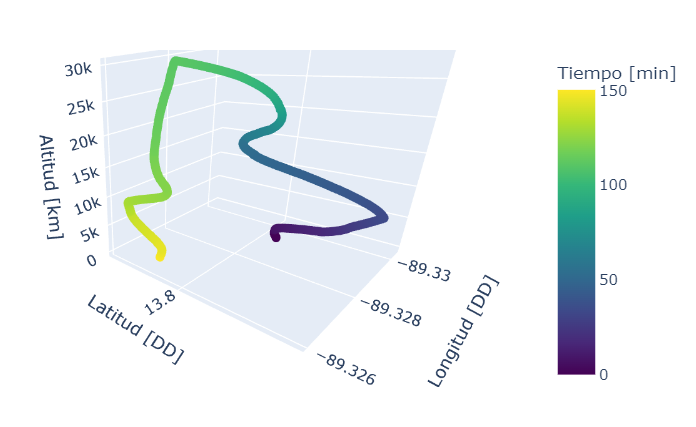
\includegraphics[width=0.75\linewidth]{document/figures/03_simu_grafico_3D_trayectoria.png}
    \caption{Vista 3D de la simulación de trayectoria}
    \label{fig:3d_trayectoria}
\end{figure}

\newpage

\begin{figure}[ht]
    \centering
    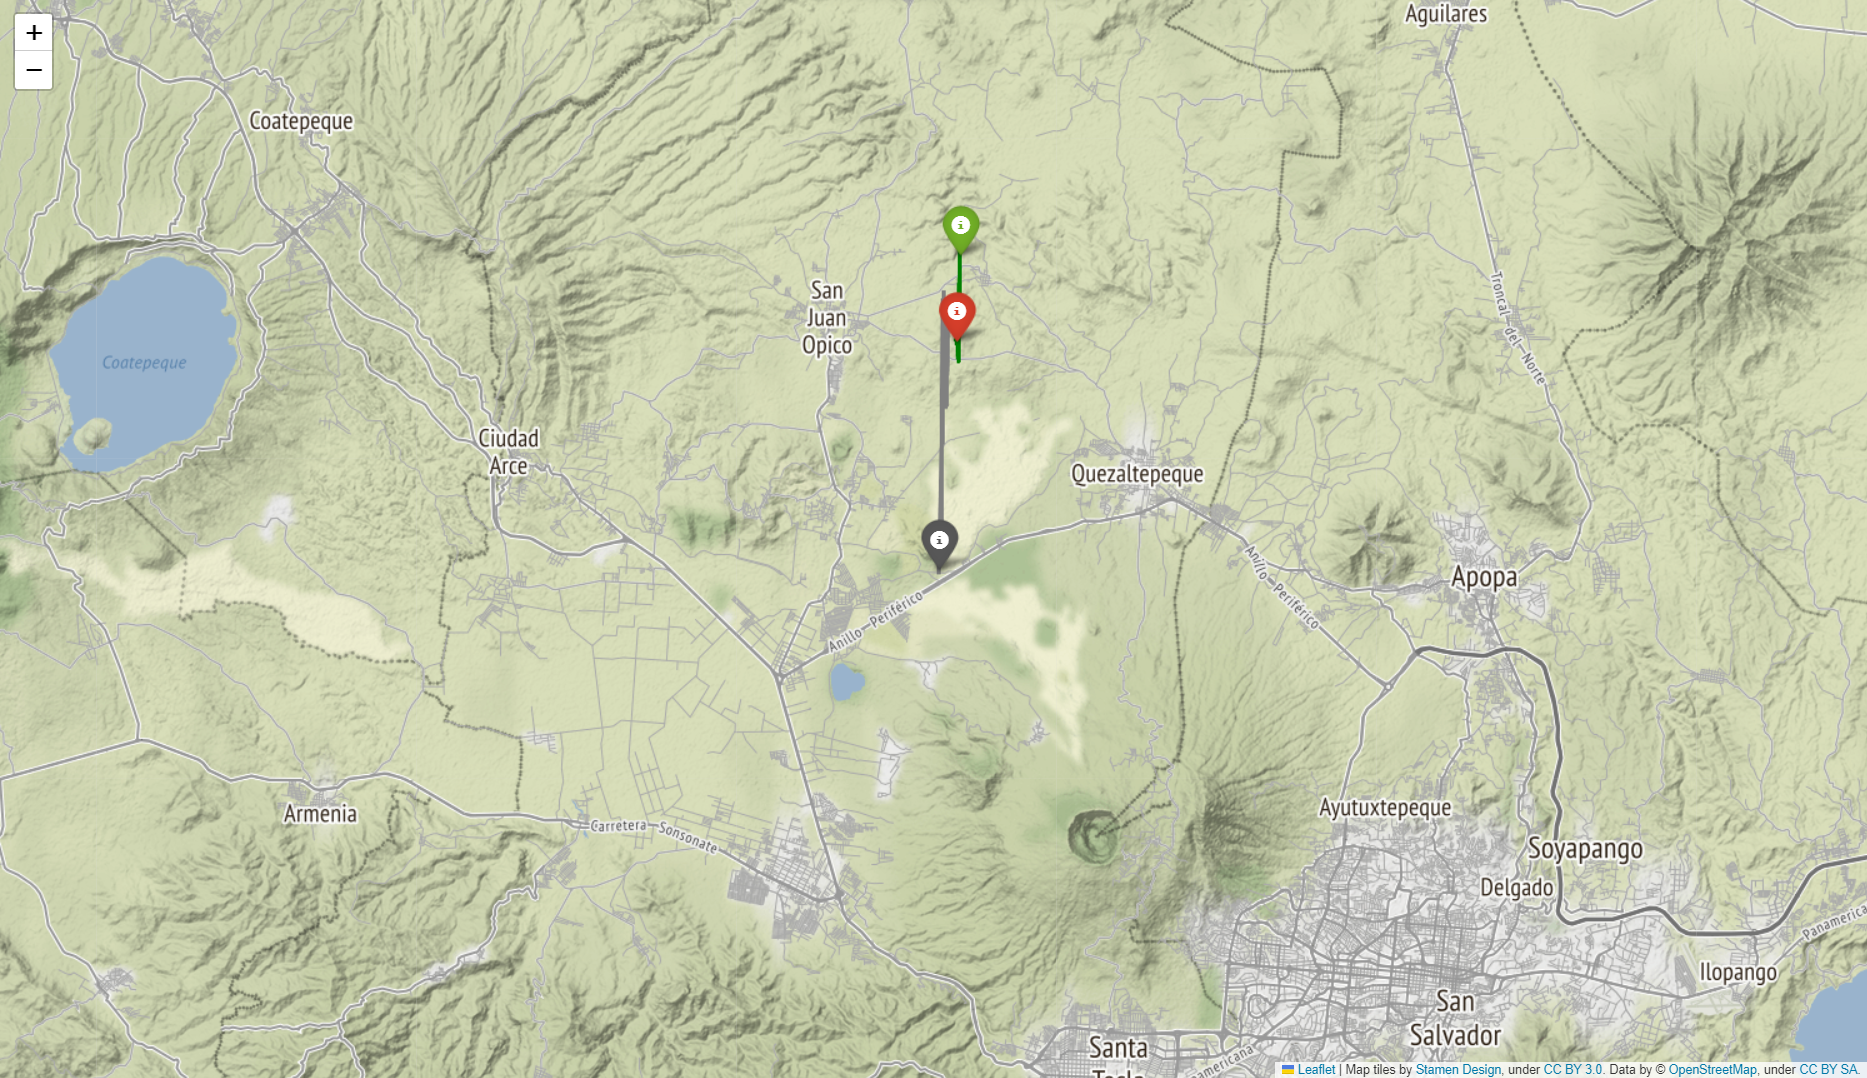
\includegraphics[width=0.9\linewidth]{document/figures/03_mapa.png}
    \caption{Vista desde un mapa geográfico de la simulación.}
    \label{fig:mapa}
\end{figure}

En figura \ref{fig:mapa} está presente la trayectoria de la sonda sobre plano horizontal que recorre distancia lineal aproximada de 9.2 km desde el punto de lanzamiento al de aterrizaje, mostrada concretamente un mapa geográfico\footnote{Se usó mapas de OpenStreet, con el módulo de Pyhton "Folium"} proporciona una visualización clara de los puntos clave de su viaje: el lugar de lanzamiento, la explosión  y el punto de aterrizaje.

\textbf{El primer punto de interés,  marcador gris}, representa el lugar de lanzamiento del globo sonda. Esta ubicación inicial es seleccionada arbitrariamente por poseer un horizonte despejado. Vale comentar, que siempre para realizar esta operación es crucial considerar las condiciones meteorológicas en el momento del lanzamiento, siendo en este trabajo obviado.

\textbf{El siguiente punto, marcador rojo}, corresponde al lugar donde tiene acción  la explosión del globo sonda y el inicio de la caída libre. Esta explosión ocurre generalmente cuando el globo ha alcanzado una altitud objetiva de la misión o cuando las características del globo son superadas por las variables atmosféricas existentes a las que fue diseñado. 

\textbf{Finalmente, el punto verde,}  índica el lugar de aterrizaje del globo sonda, este es el punto más crucial y es necesario una precisión aceptable de simulación para determinar una recuperación exitosa del globo sonda y los instrumento que transporte.

\newpage

\begin{figure}[ht]
    \centering
    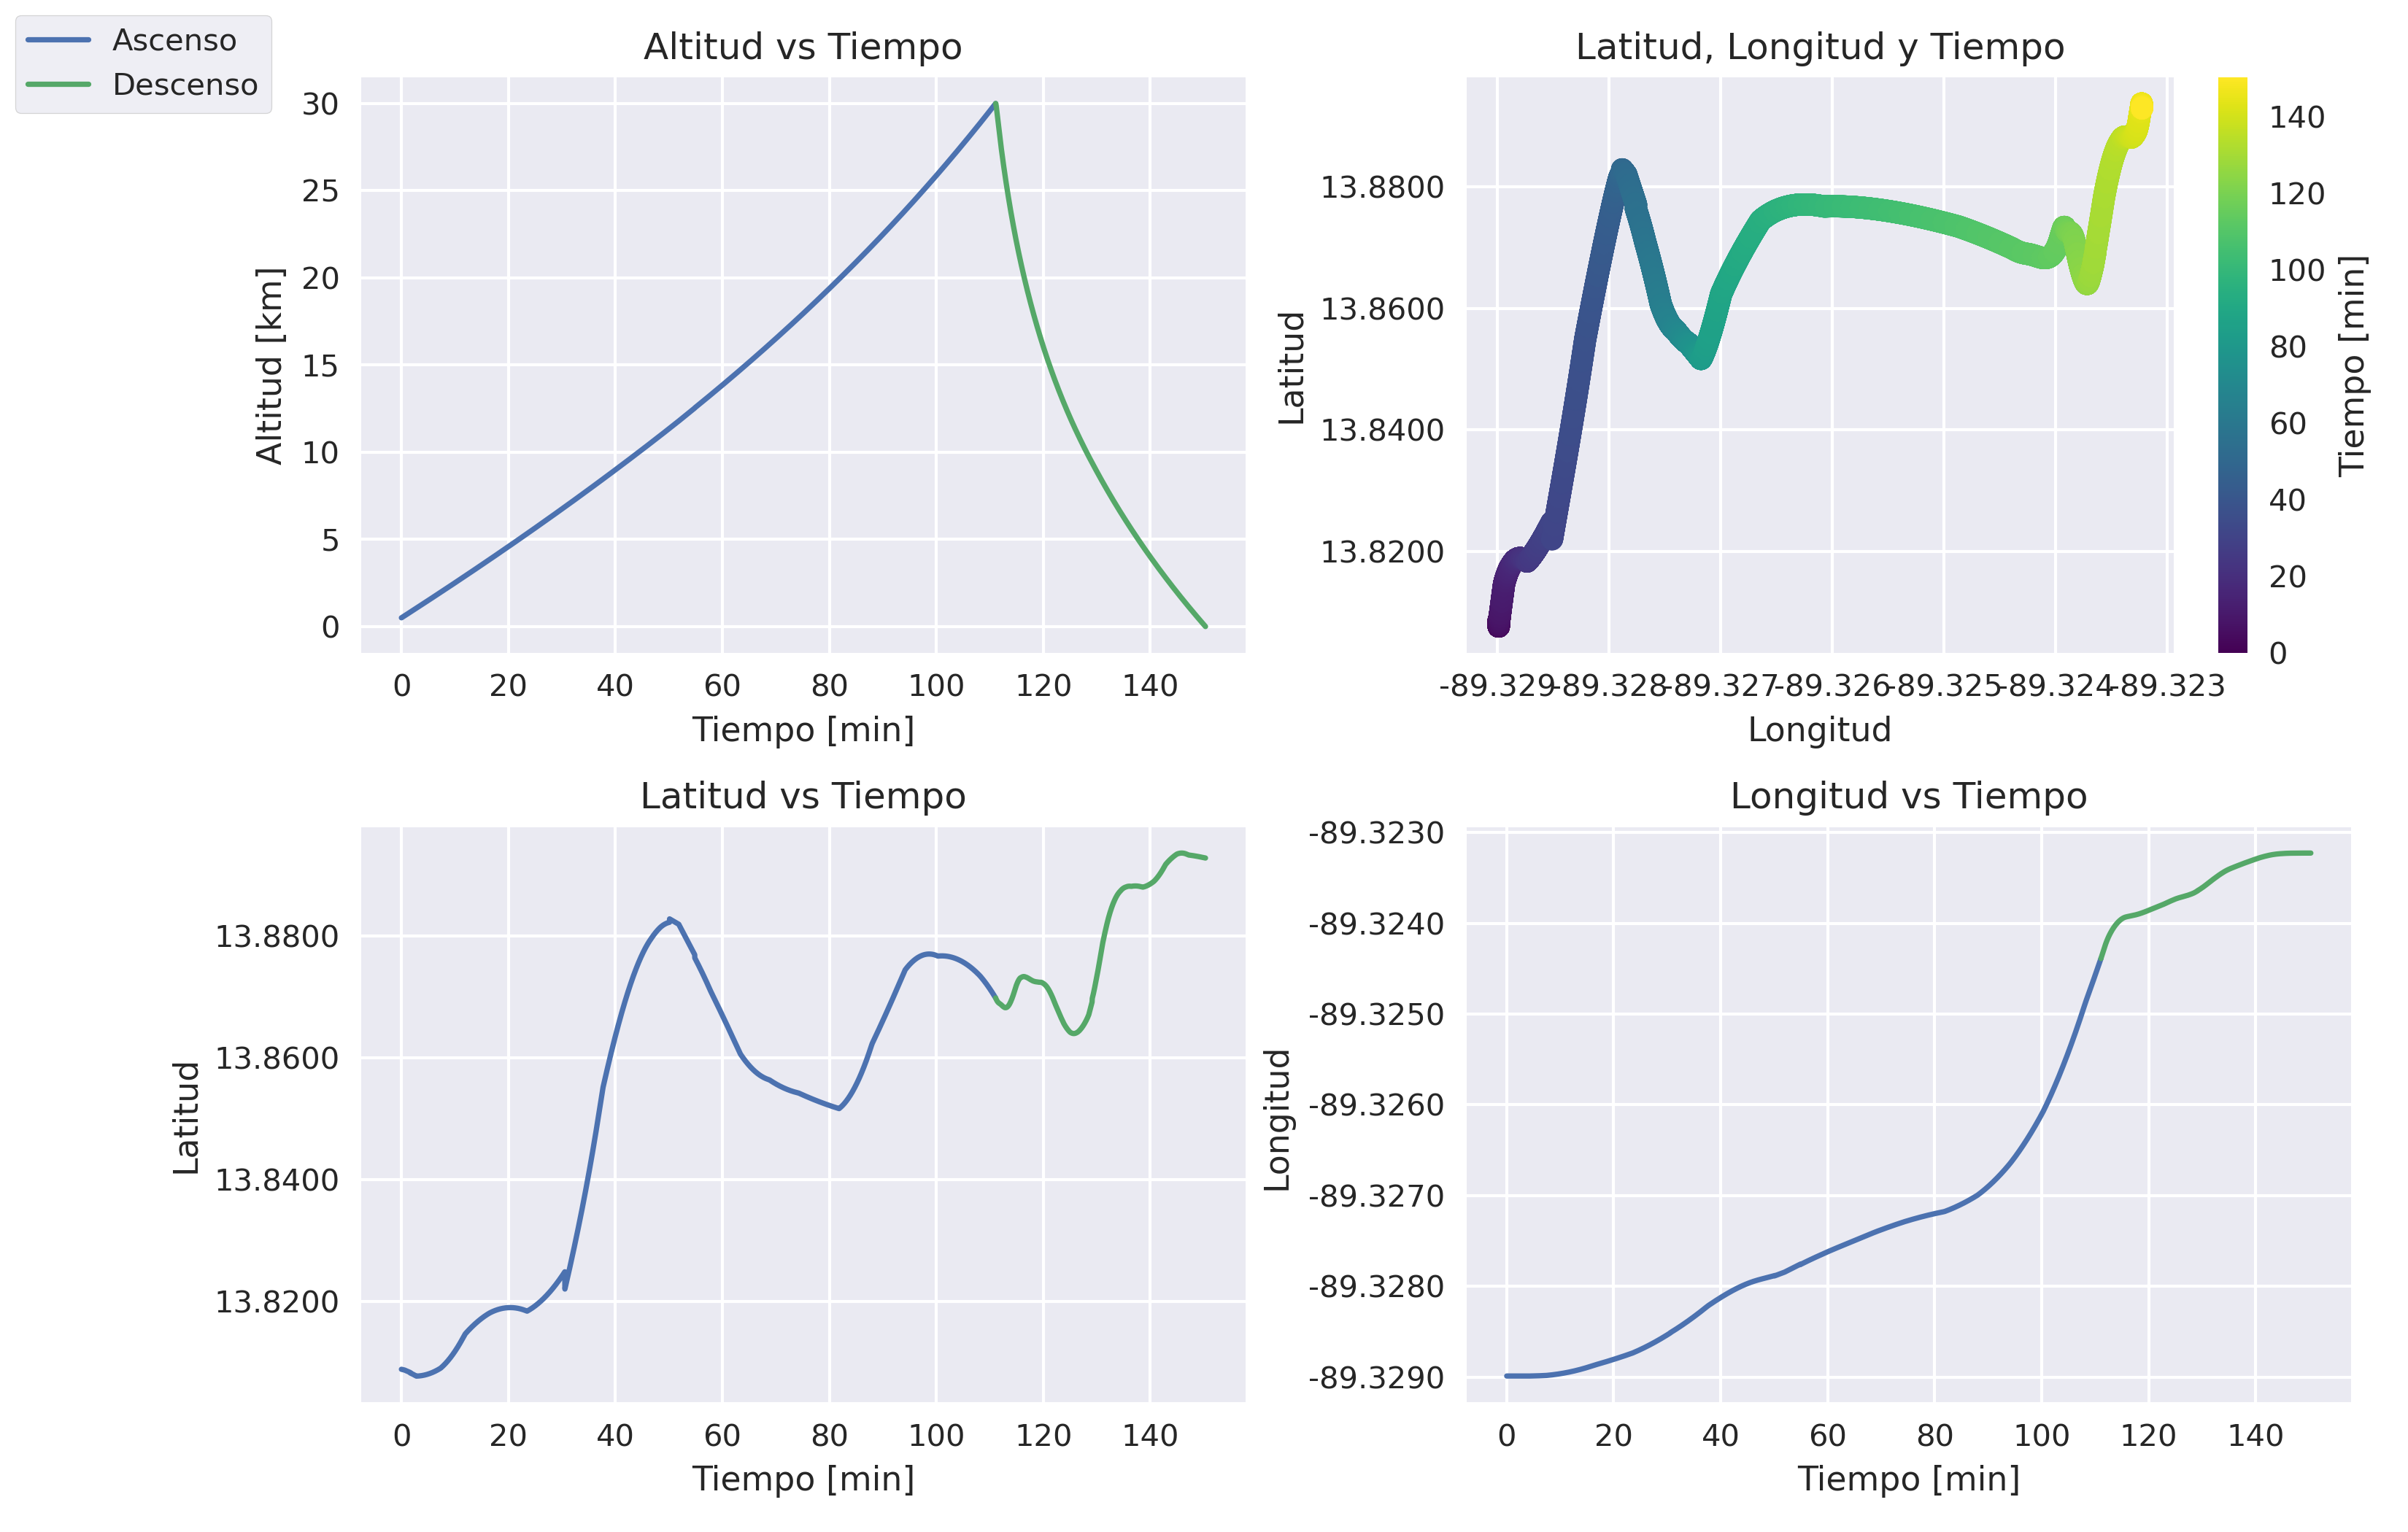
\includegraphics[width=0.93\linewidth]{document/figures/03_plano_posicion_vs_tiempo.png}
    \caption{Vista desde un plano de la posición y tiempo}
    \label{fig:posicion_vs_tiempo}
\end{figure}

Se efectuó una inspección del fenómeno posición vs tiempo, mostrándose  dividido en gráficos que se muestra en figura \ref{fig:posicion_vs_tiempo}. Acto seguido, se procede a detallar: 

\textbf{En la primera subgráfica Altitud vs Tiempo},  se observa una curva ascendente seguida de una curva descendente, ambas suaves y graduales. Además, en la zona del ascenso posee  el mayor tiempo  de 111 minutos, su descenso es lo que menos toma tiempo 39 minutos,  esto señala que aproximadamente 3/4  es el tiempo de subida y 1/4 descenso.

\textbf{En la segunda subgráfica Latitud, Longitud y Tiempo}, donde se muestra la latitud y la longitud con trazos pintados que representar la trayectoria recorrida a medida que pasa el tiempo. La forma de los trazos y su dirección indican curvas suaves y  cambios bruscos de dirección aleatorios.

\textbf{En la tercera y en la cuarta subgráfica, Latitud vs Tiempo y Longitud vs Tiempo respectivamente}, ambas presentan curvas con cambios a medida que transcurre el tiempo. Sin embargo, se muestra la latitud en comparación con la longitud tiene una mayor variación y traslación en función del tiempo, véase figura \ref{fig:mapa} para observar mejor esta situación; llama mucho la atención esta tendencia en el movimiento porque podría sugerir vientos en latitud o específicamente la componente de viento U dominantes.

\newpage

\begin{figure}[ht]
    \centering
    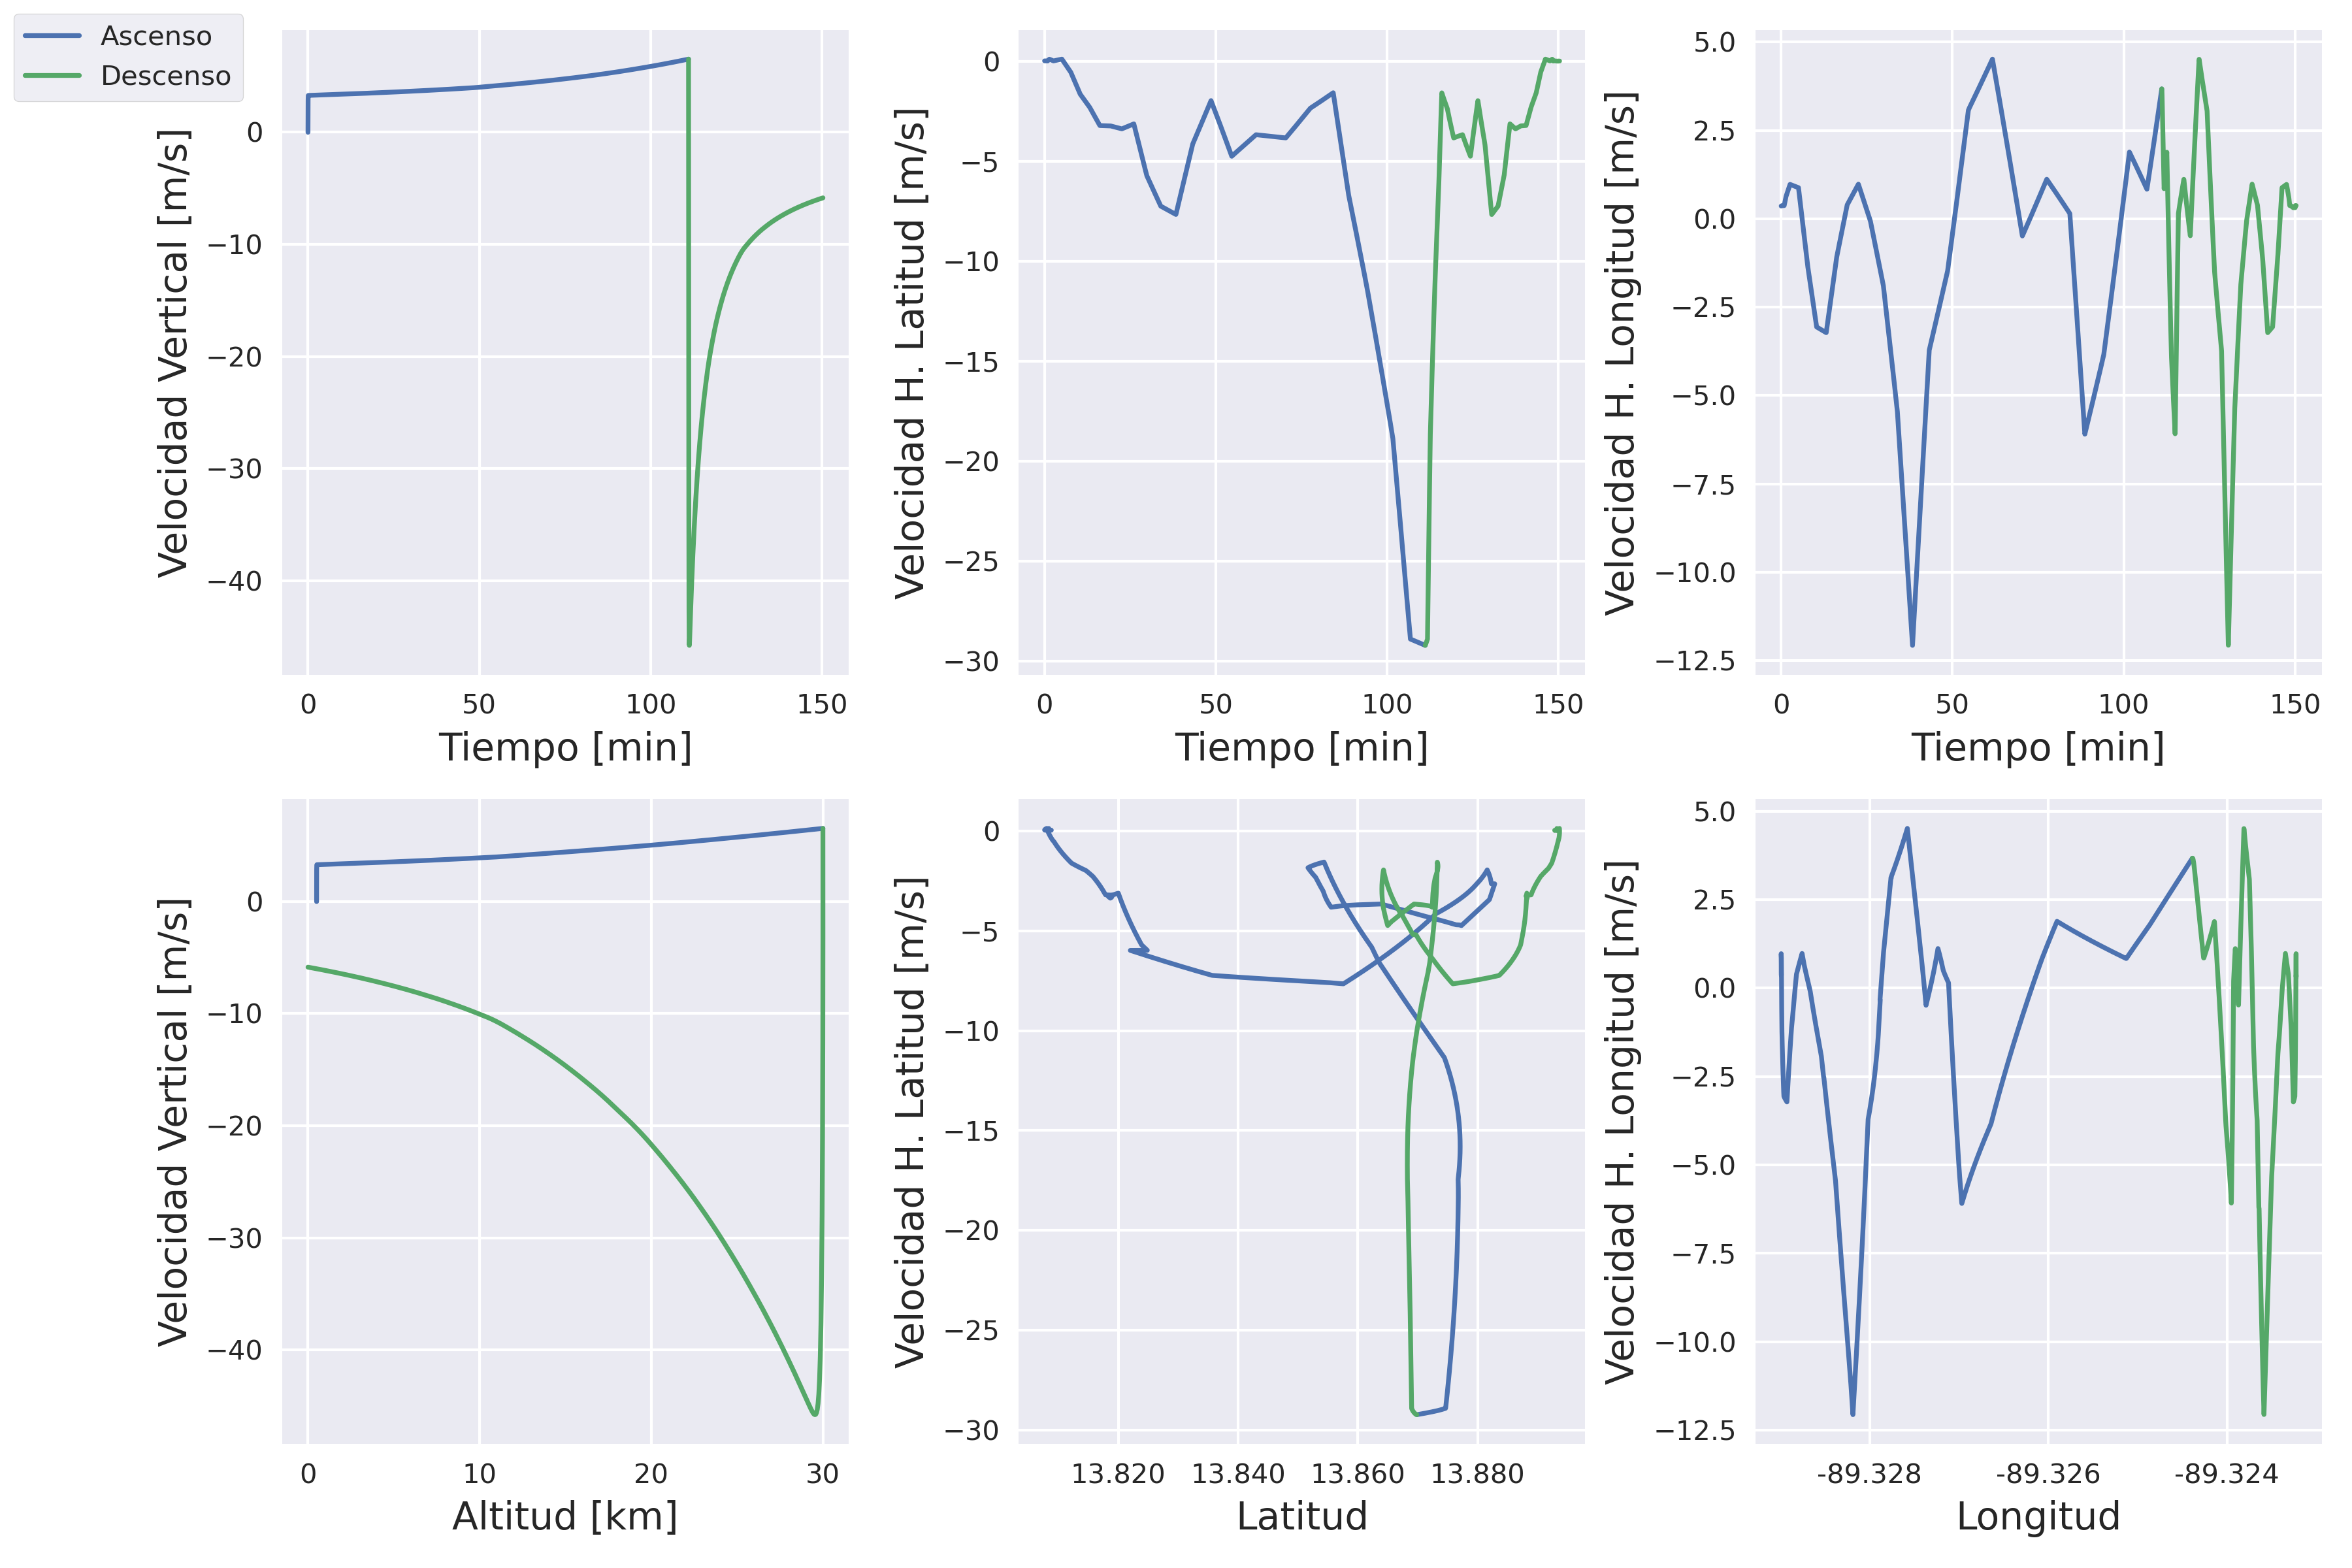
\includegraphics[width=0.77\linewidth]{document/figures/03_graficas_tiempo_altitud_vs_velocidad.png}
    \caption{Gráficas de velocidades vs posición y tiempo}
    \label{fig:velocidades_posicon_y_tiempo}
\end{figure}

\small
En figura \ref{fig:velocidades_posicon_y_tiempo} se visualiza  tres tipos de velocidades, una vertical y dos horizontales que representan la altitud, latitud y longitud. Se expone los resultados obtenidos divididos en las dos componentes del movimiento vertical y horizontal:

\begin{itemize}
    \item \textbf{Velocidad vertical respecto al tiempo y posición:}     
        \begin{itemize}
            \item En las gráficas  existe un comportamiento de aumento gradual y también bastante asintótico tanto en el tiempo como en altitud en el momento del asenso y como si se tratase de acercarse a un valor límite sin llegar a alcanzarlo, y tal como sugirió el análisis descriptivo de un promedio de 4.4 m/s con una desviación típica con baja variabilidad de 0.90 m/s. El descenso muestra una desaceleración como si de un logaritmo inverso se tratase, y se observa que el objeto al momento de impactar con la superficie de la tierra en la colisión presenta una rapidez  de  $- \;  5.9$  m/s, esto es efecto del paracaídas principalmente y la densidad atmosférica. Es notable, la velocidad luego de la explosión es dramática, pero es un comportamiento normal de un sistema bajo los efectos de caída libre que no parte del reposo.
        \end{itemize}

    \item \textbf{Velocidad horizontal en latitud y longitud respecto al tiempo y posición:}
    \begin{itemize}         
        \item A medida que el tiempo y la posición avanza, el globo se desplaza con ciertas velocidades a lo largo de diferentes latitudes y longitudes, lo cual se refleja en la variación en las gráficas que presentan fluctuaciones y oscilaciones. 
        \item Se observó que existencia tendencias anormales en el que las velocidades con respecto al tiempo y la posición geográfica sugiere un comportamiento simétrico cuando debería existir más aleatoriedad. Esta información recuerda a la poca variación que mostró en el análisis descriptivo.  
    \end{itemize}

\end{itemize}
\normalsize

\newpage

\subsection{Geometría del globo vs posición y tiempo}

Conforme en ecuación \ref{eq:radio} se realizaron los cálculos para ver como este fenómeno evoluciona en función del tiempo y la altura. 

\begin{figure}[H]
    \centering
    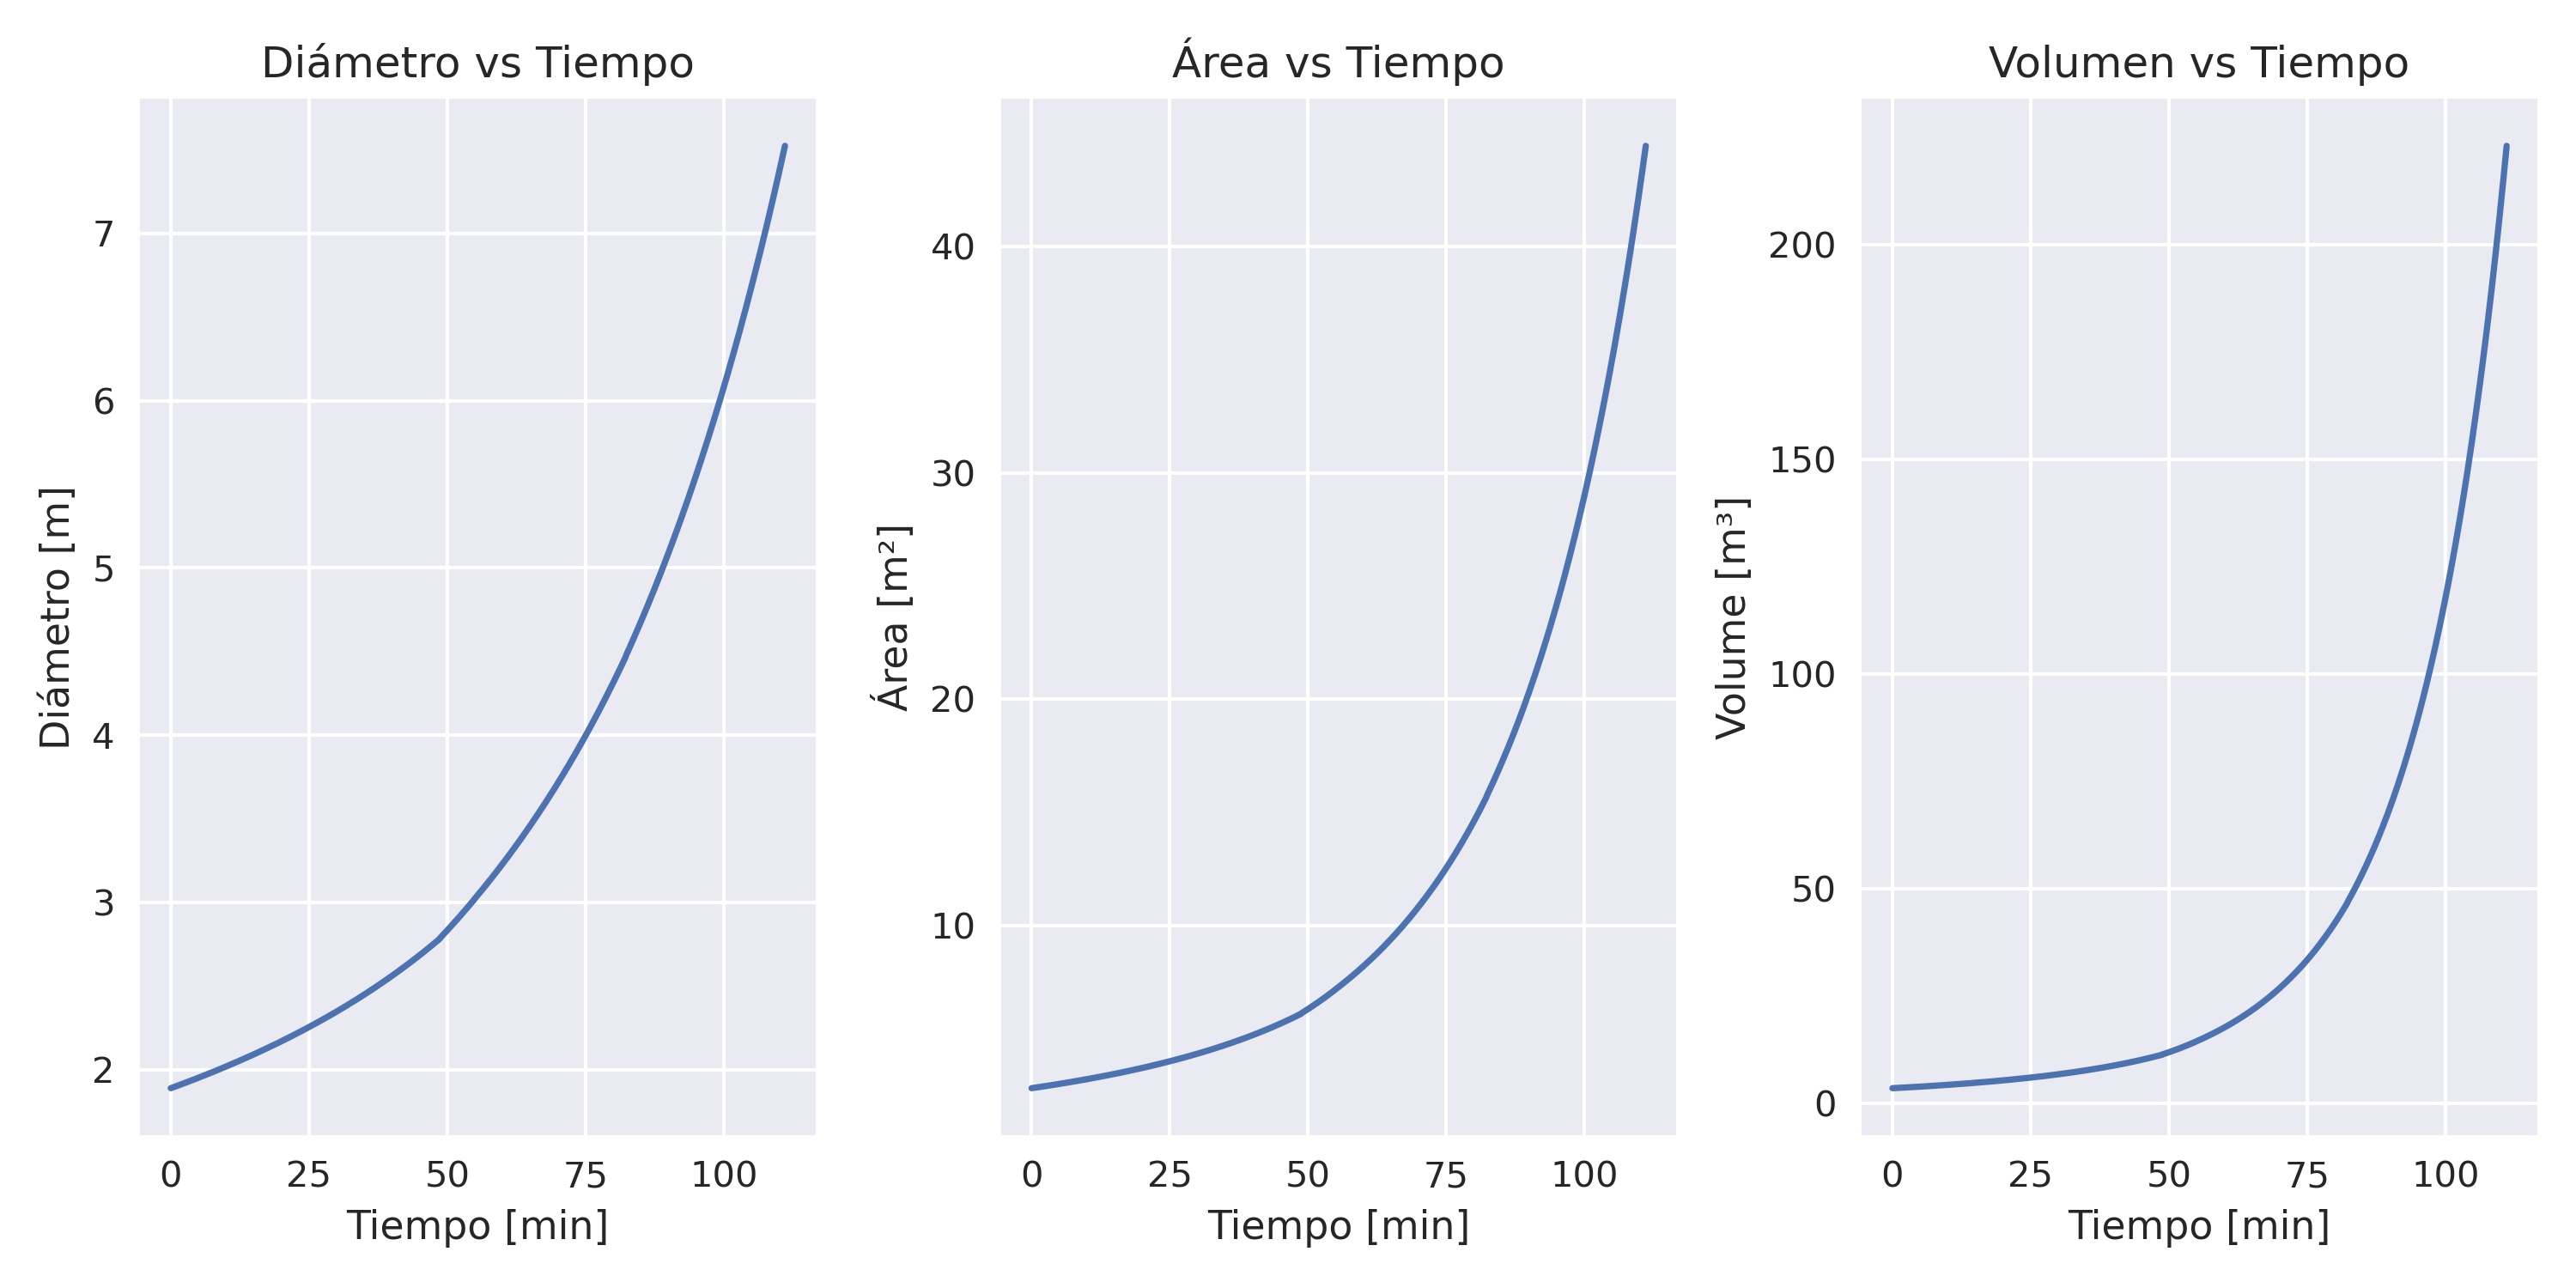
\includegraphics[width=0.9\linewidth]{document/figures/03_geometria_vs_tiempo.png}
    \caption{Geometría en función del tiempo}
    \label{fig:geometria_vs_tiempo}
\end{figure}

\begin{figure}[H]
    \centering
    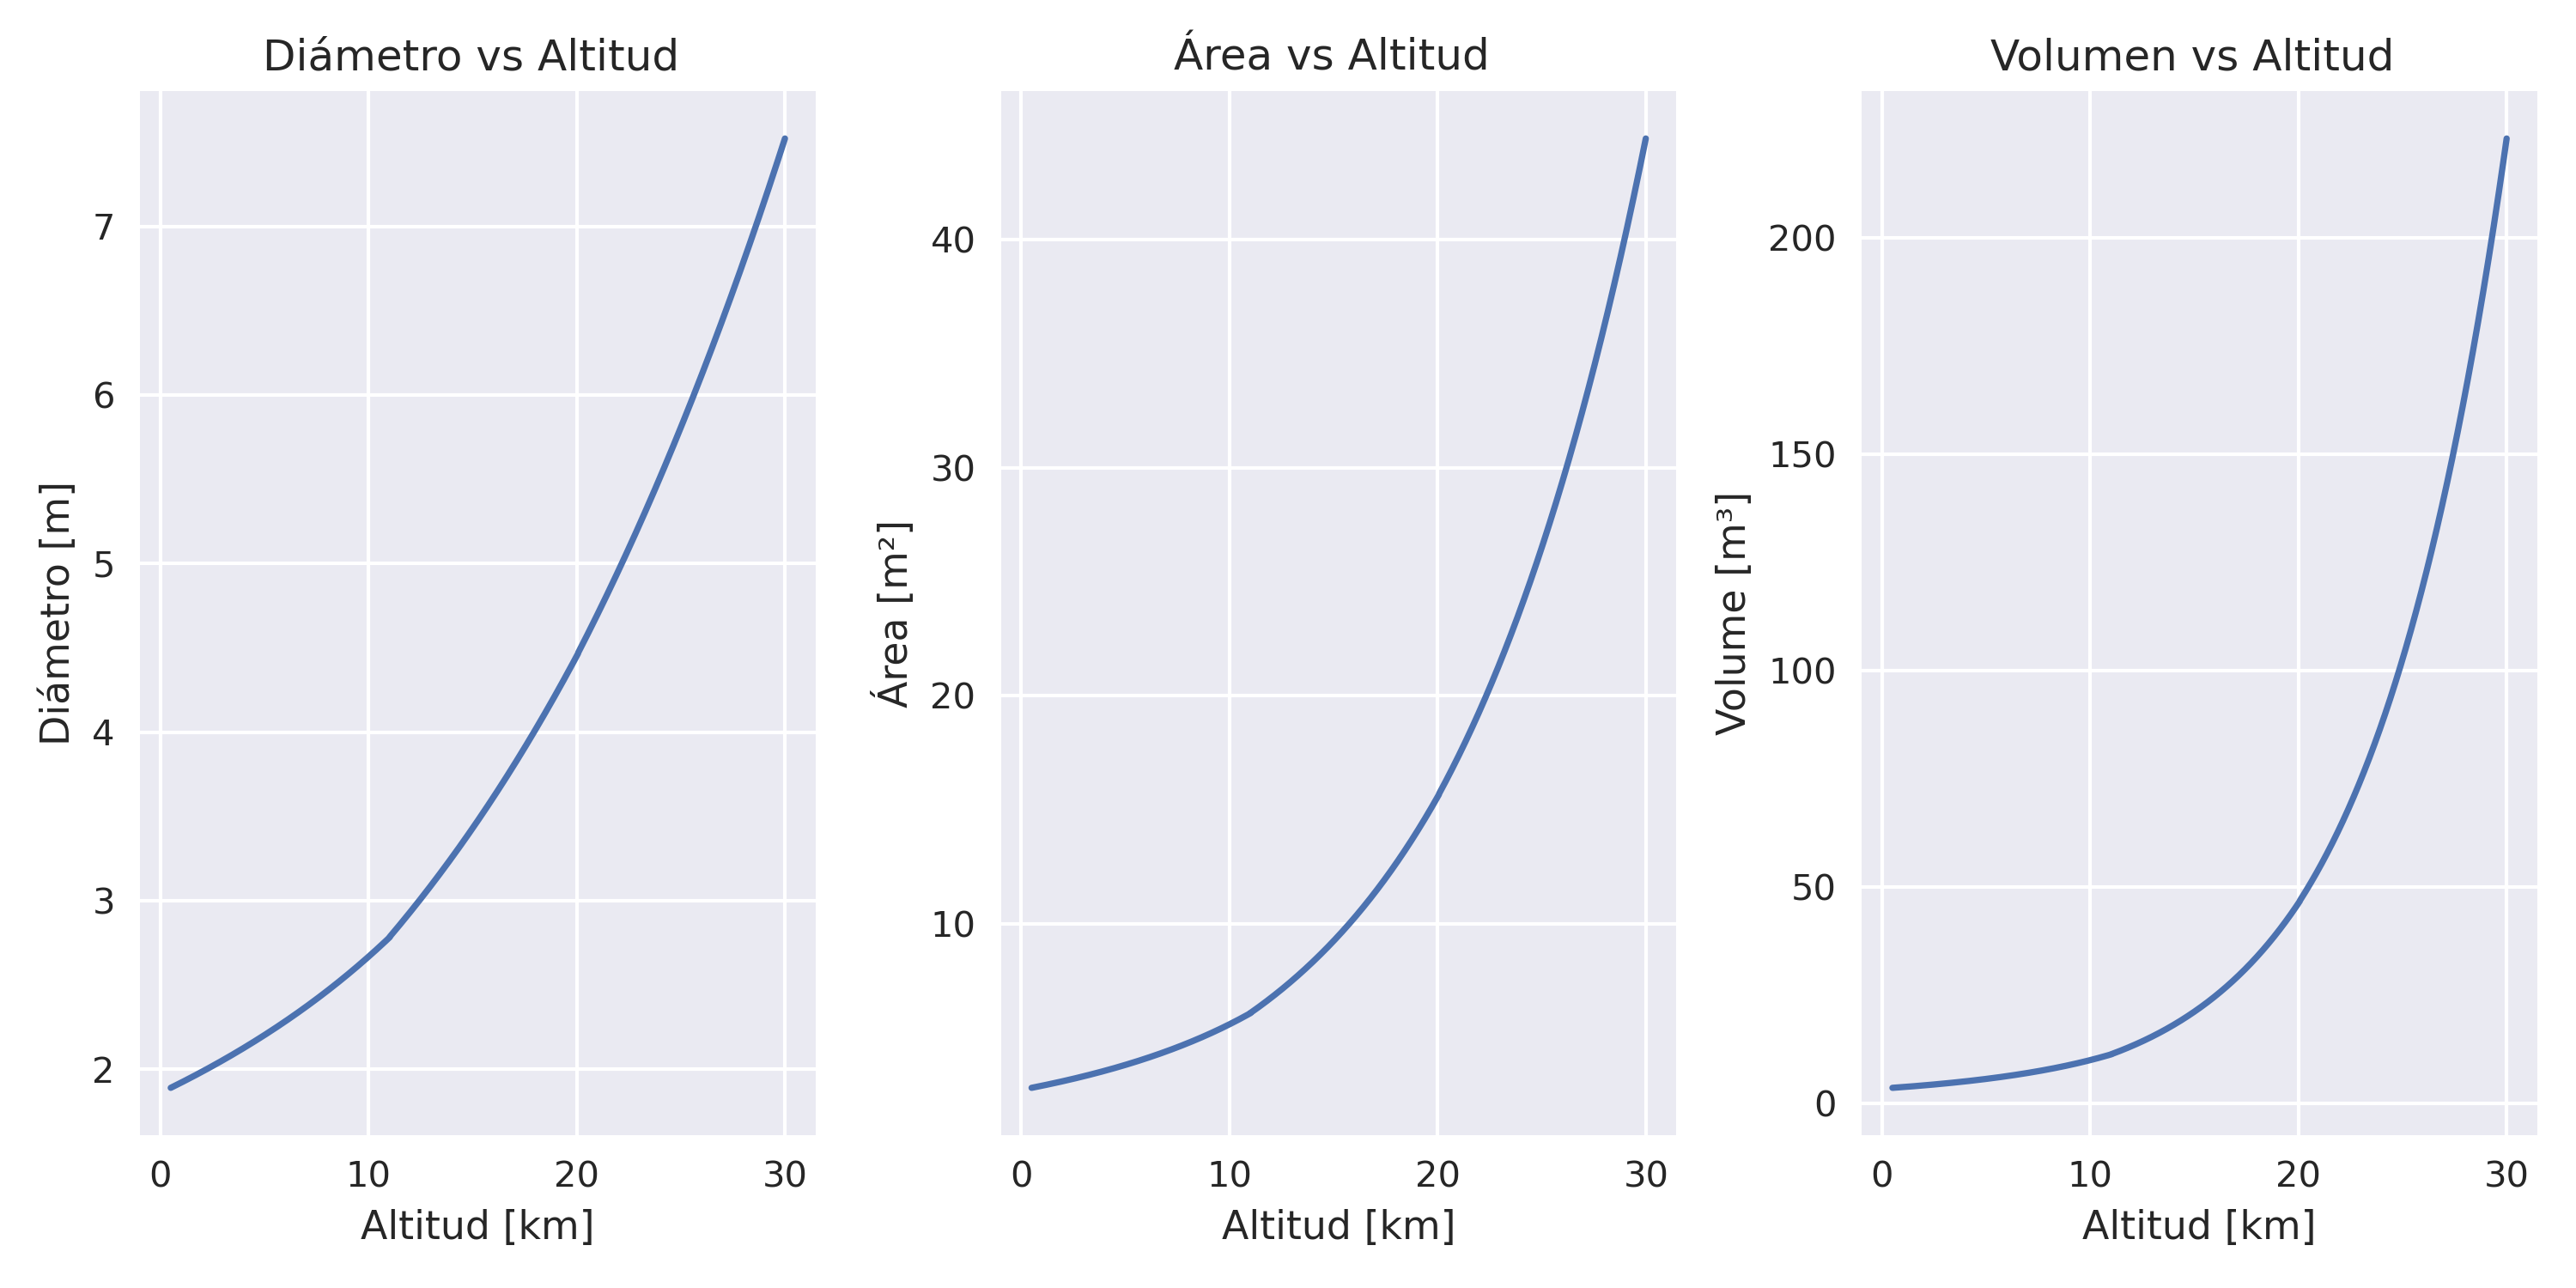
\includegraphics[width=0.92\linewidth]{document/figures/03_geometria_vs_altitud.png}
    \caption{Geometría en función de la altitud}
    \label{fig:geometria_vs_altitud}
\end{figure}

\newpage

Los resultados obtenidos en figura \ref{fig:geometria_vs_tiempo} y \ref{fig:geometria_vs_altitud}  modelan que el globo aproximadamente cambian su geometría bruscamente  después de los 12 km y 50 min, crecimiento más aceleradamente partir de ese momento. Generalmente, todas las gráficas tiene una forma exponencial, la razón de este comportamiento es que el área y el volumen depende del diámetro de globo y este último a su vez depende de las condiciones atmosféricas presentes en diferentes altitudes que cambia al transcurso del tiempo.

\begin{figure}[h]
    \centering
    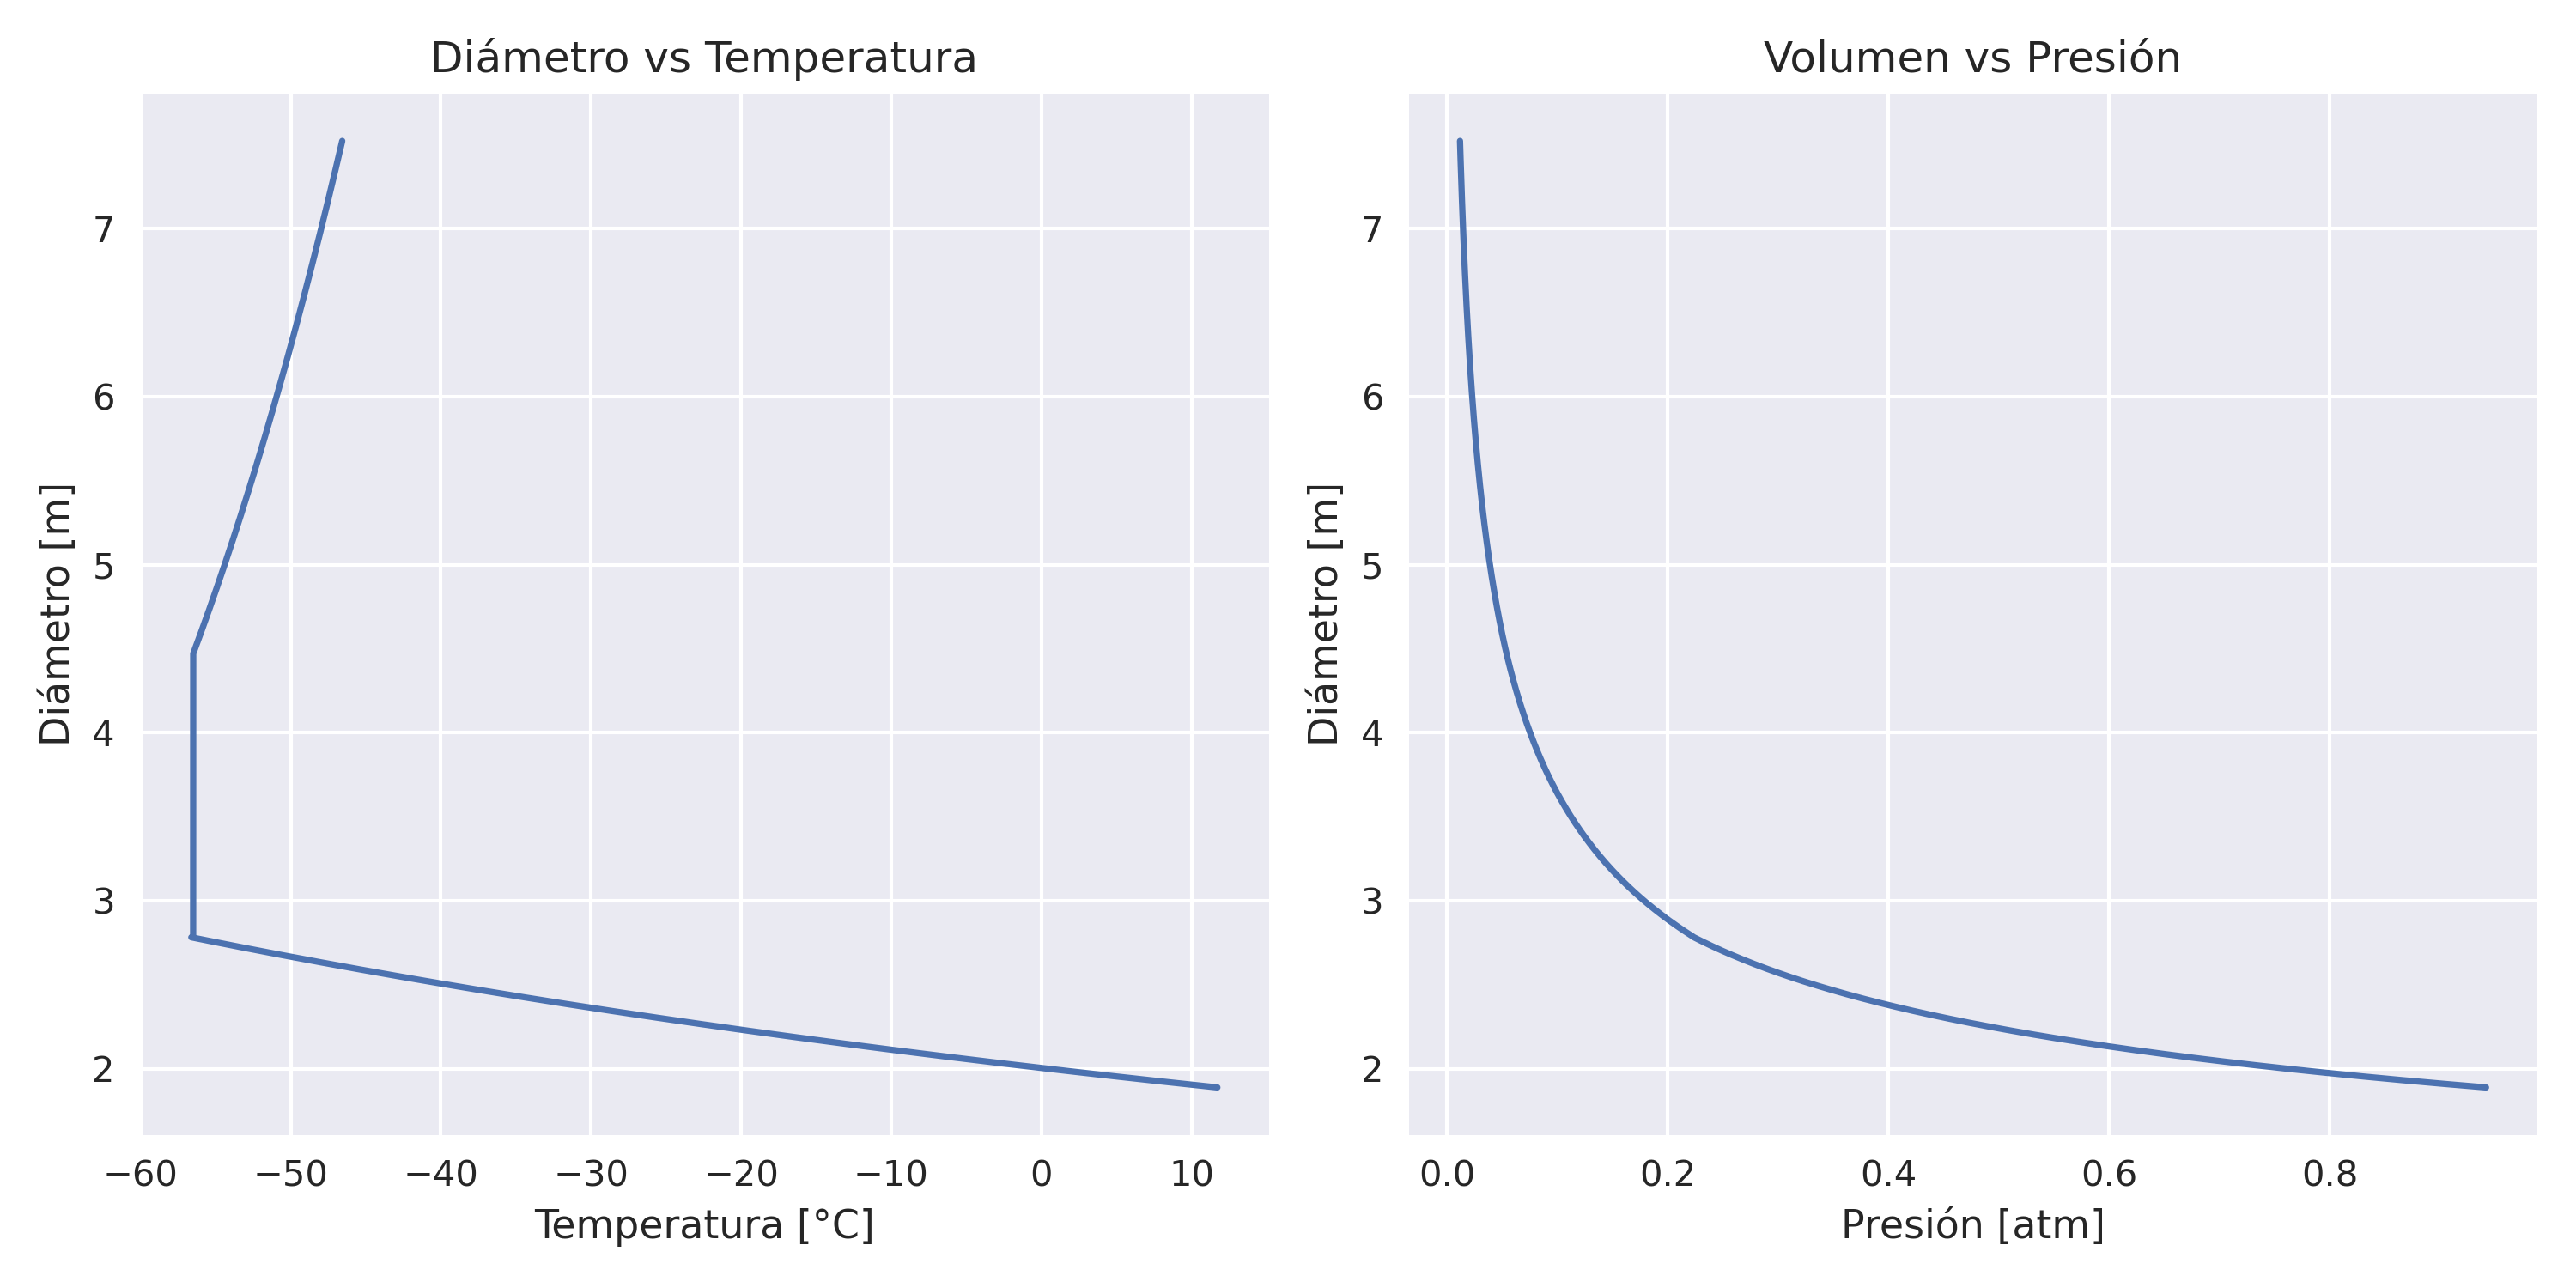
\includegraphics[width=1\linewidth]{document/figures/03_geometria_vs_atmosfera.png}
    \caption{Geometría en función del tiempo}
    \label{fig:geometria_vs_atmosferica}
\end{figure}

Cuando se analiza el diámetro en función de las variables atmosféricas presentes de la ecuación \ref{eq:radio}  como se muestra en la figura \ref{fig:geometria_vs_atmosferica} observamos que la temperatura no es tan significativa en el aporte al crecimiento del diámetro a diferencia de la caída de presión al ascender en la atmósfera quién es la causante de la explosión del globo, por lo tanto,  cuando se estime la cantidad del gas de elevación se debe de tener espacial cuidado en la cantidad  de gas porque determinará la altitud máxima debido a la presión.

La altitud y longitud no presenta ninguna relación con la geometría, esa es la razón por la que no existe ninguna gráfica con respecto a estas variables ni de las demás del conjunto de datos.

\newpage

\subsection{Atmosféricos vs posición y tiempo}

Al analizar los resultados de figura \ref{fig:atmosferica_altitud}, se observa que la relación entre la temperatura y la altitud presenta un comportamiento lineal seccionado. El primer tramo muestra una pendiente de  -6.5 °C/km, la cual está altamente influenciada por la transferencia de calor por convección, lo que sugiere que es el tramo donde los componentes electrónicos estarán bajo el mayor estrés térmico \cite{TASEC_Lab}. Posteriormente, se alcanza una región intermedia isotérmica entre los  11 km y 20 km y luego se produce un tramo final con una pendiente de +2.8 °C/km hasta llegar a los 30 km\footnote{Recuérdese, que los delta de temperatura de Kelvin y Celsius son directos}. Estas condiciones son críticas para cualquier sistema electrónico involucrado y la estructura de la sonda.

Continuando con figura \ref{fig:atmosferica_altitud},  en la presión y densidad, se puede apreciar un comportamiento exponencial en decadencia, teniendo en el caso de la densidad valores límite de 0.01845 kg/m³, para la presión 0.000118431 atm (12 hPa). Por último, la gravedad varía de forma lineal inversamente proporcional a la altura con una pendiente de --0.003056 $\frac{m}{s^{2}}$/$km$ .

\begin{figure}[h]
    \centering
    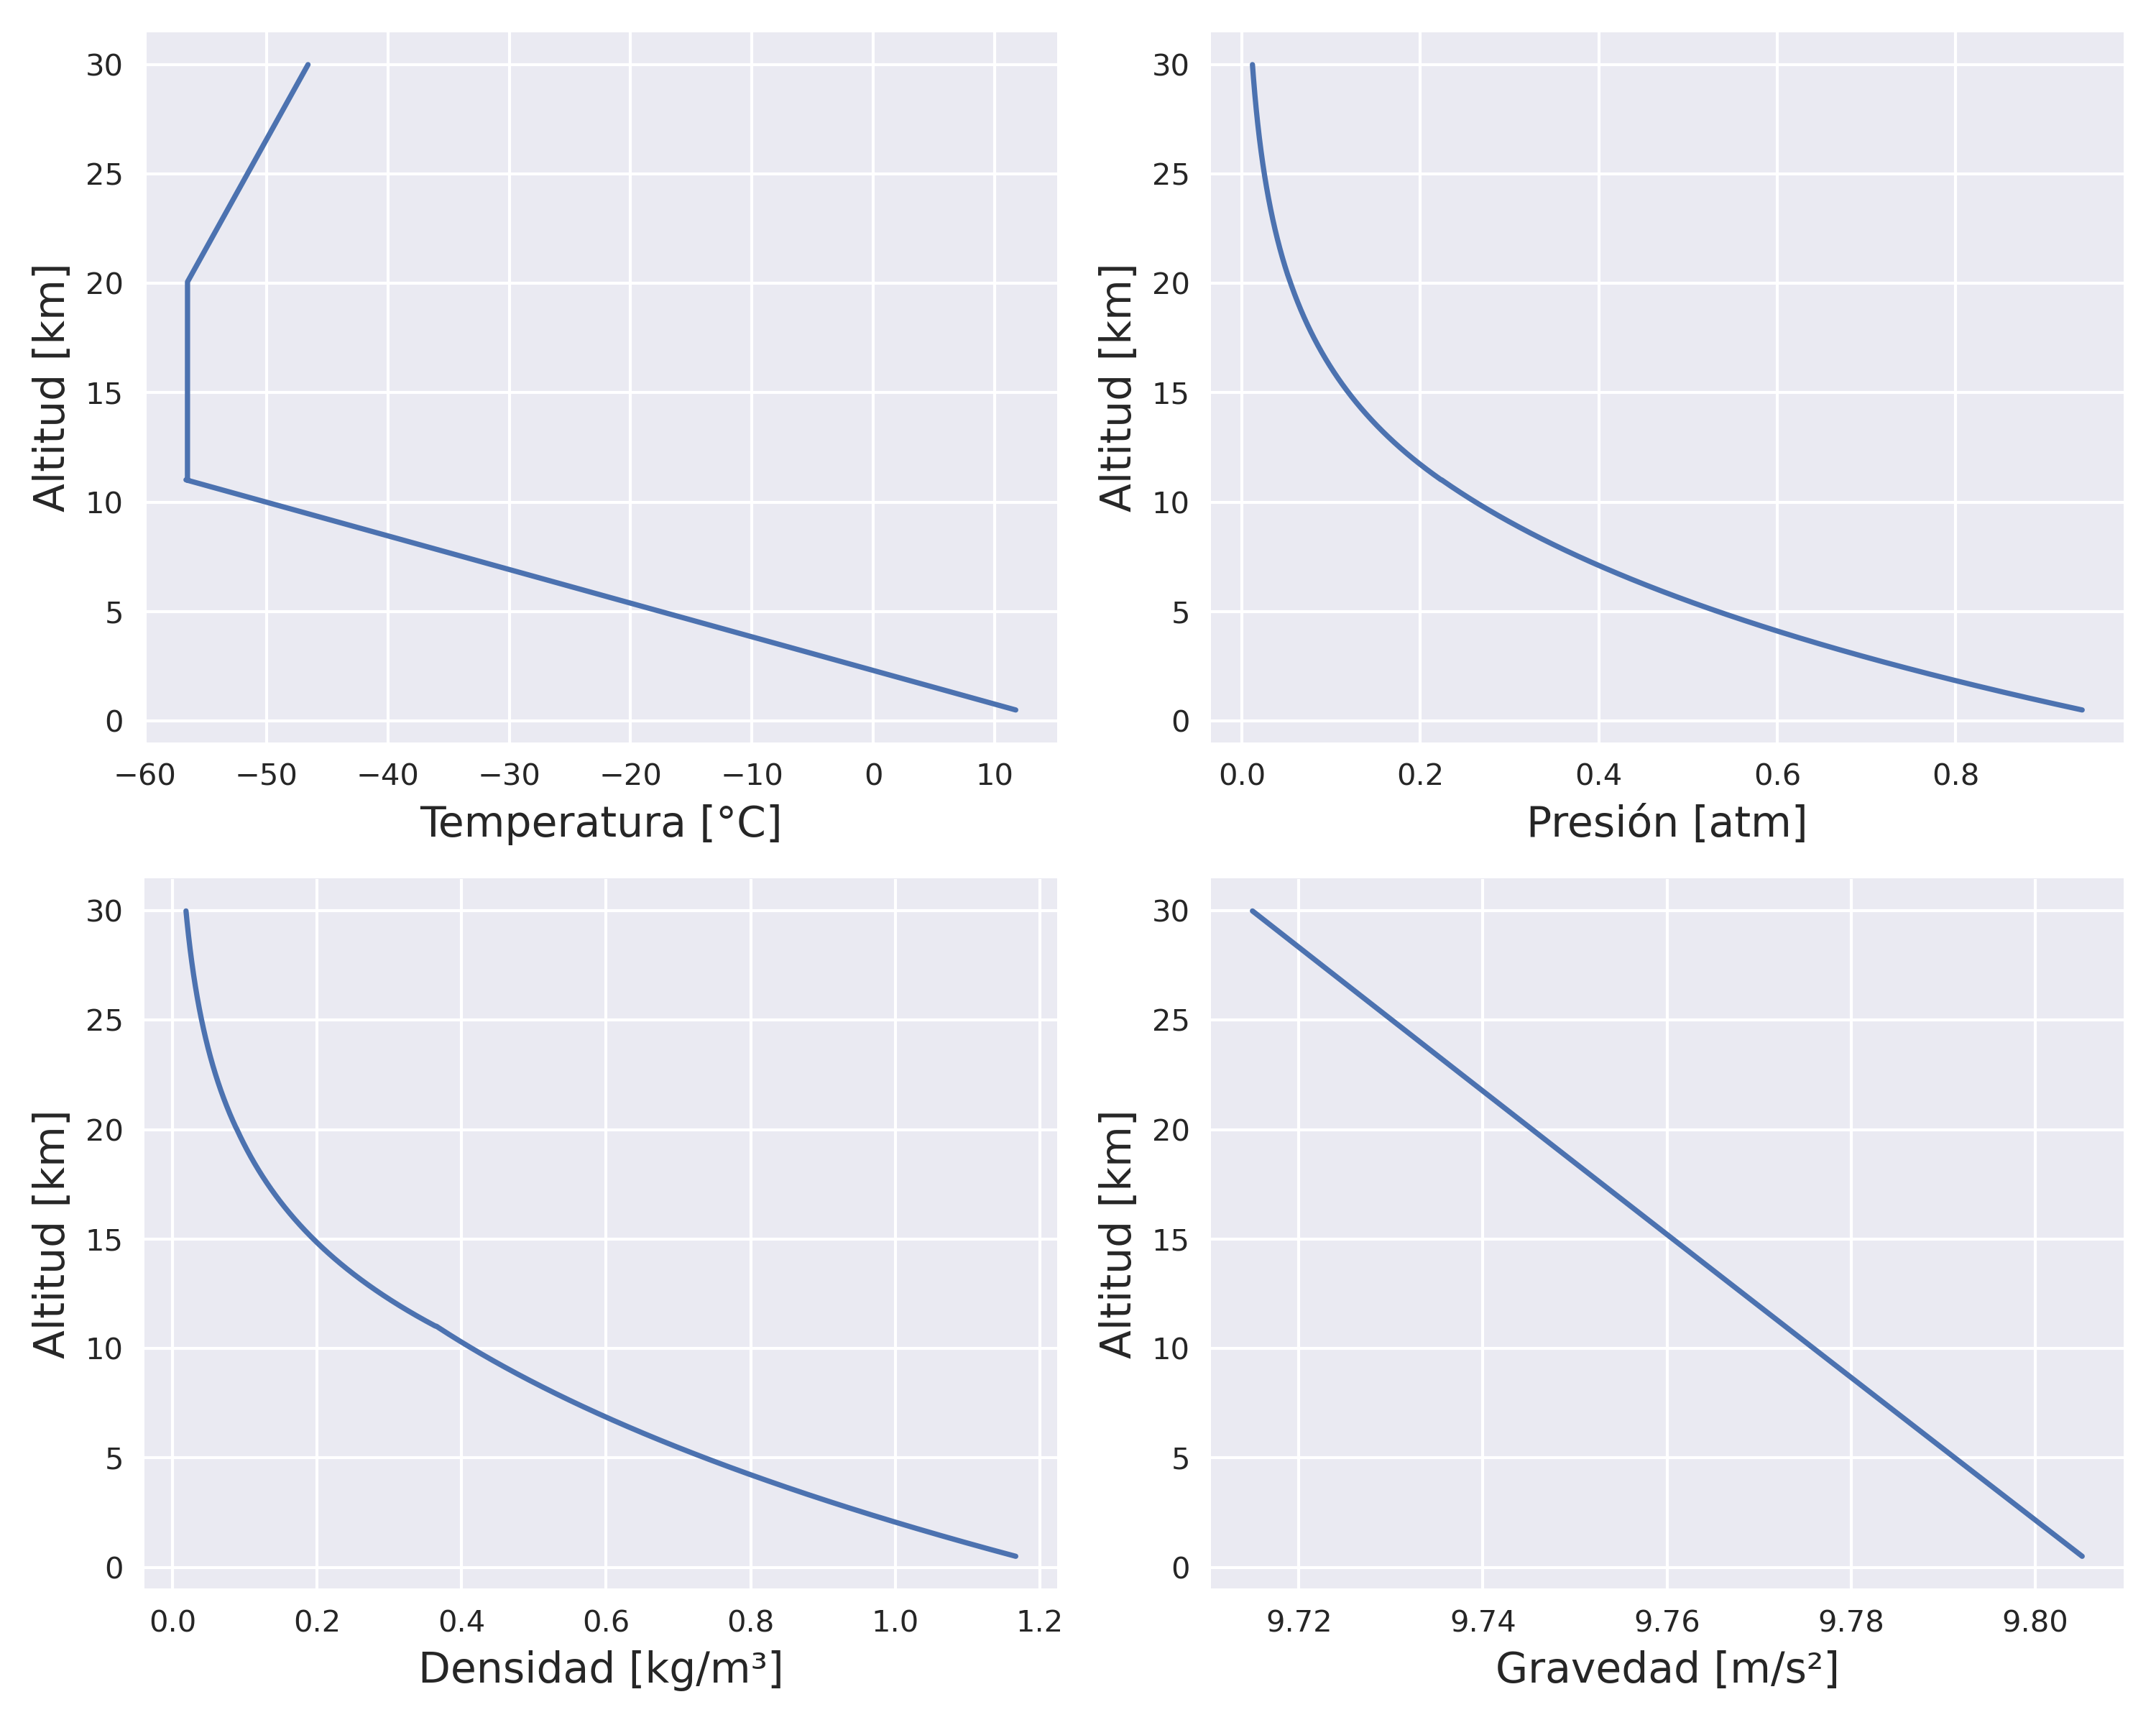
\includegraphics[width=0.85\linewidth]{document/figures/03_atmsferica_vs_altitud.png}
    \caption{Variables atmosféricas respecto a la altitud}
    \label{fig:atmosferica_altitud}
\end{figure}

\newpage

\begin{figure}[!t]
    \centering
    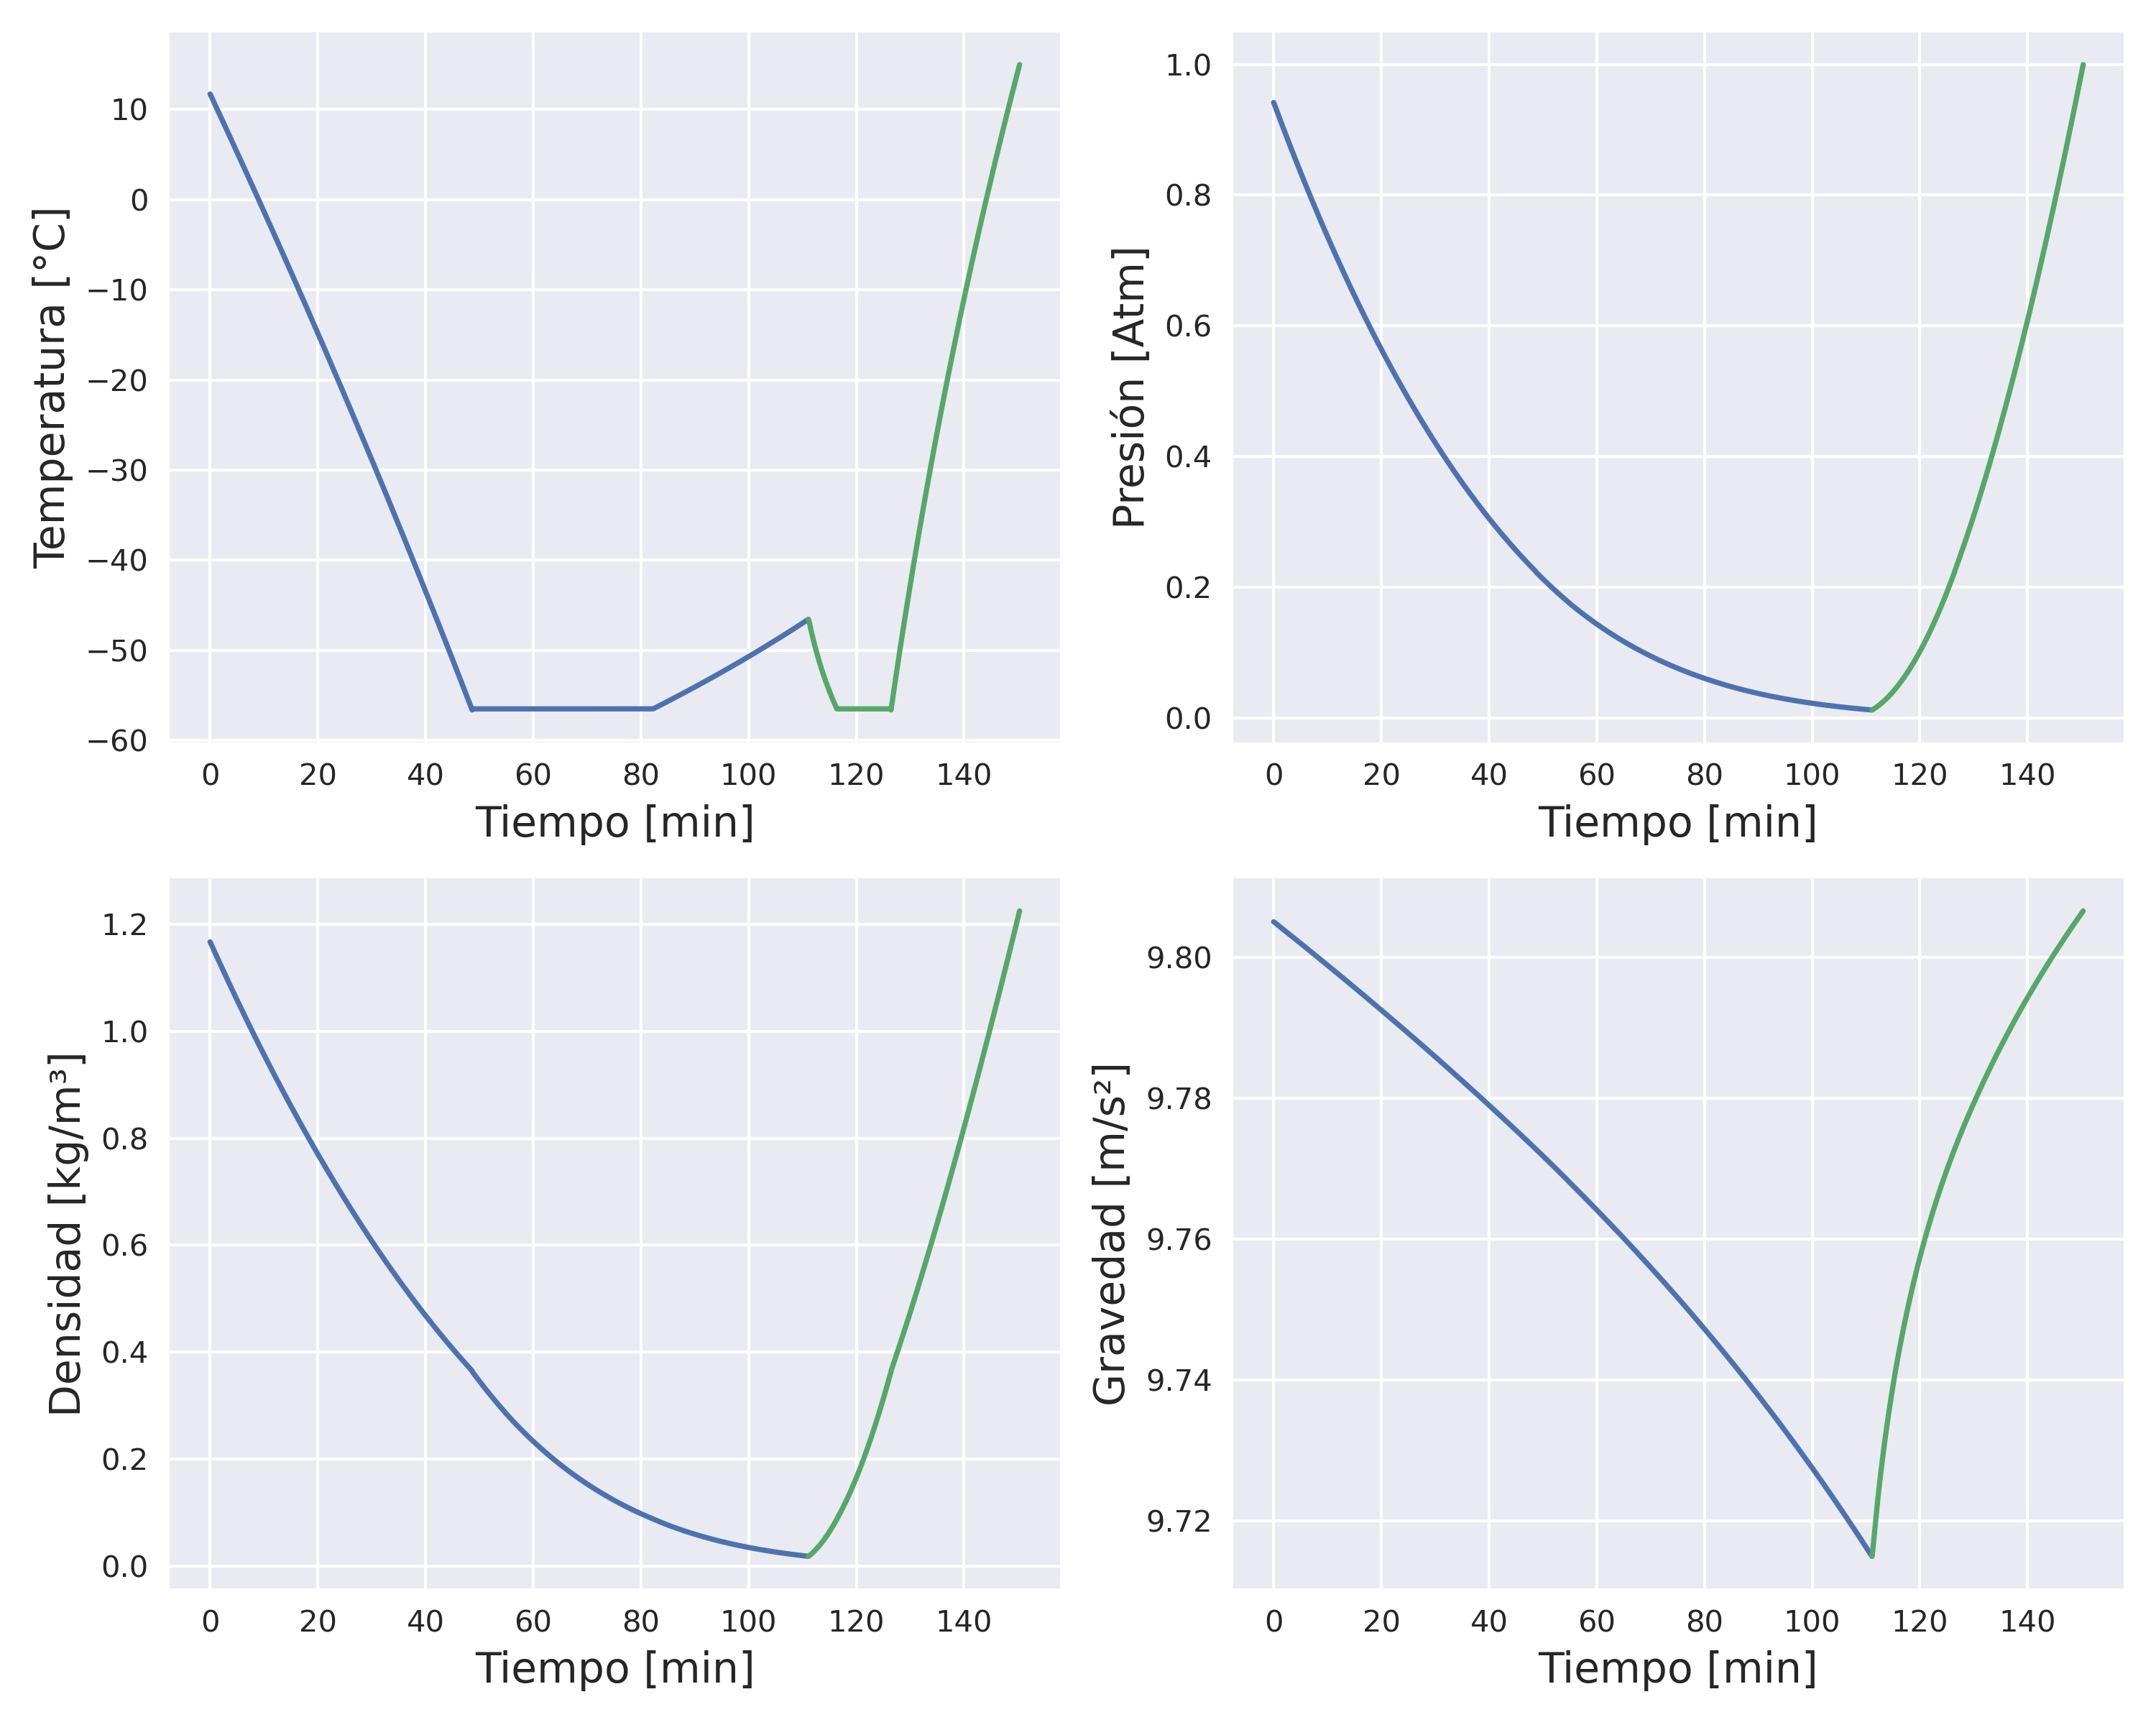
\includegraphics[width=0.75\linewidth]{document/figures/03_atmsferica_vs_tiempo.png}
    \caption{Variables atmosféricas respecto al tiempo}
    \label{fig:atmosferica_tiempo}
\end{figure}

Una vez que se relaciona el tiempo con cada variable atmosférico, como en figura \ref{fig:atmosferica_tiempo}, es posible discernir claramente las condiciones de riesgo asociadas a las tasas de cambio bruscas, especialmente en el caso de la temperatura y la presión, las cuales son las que podrían afectar a los materiales y/o componentes electrónicos en la misión.

Al analizar la curva de temperatura en función del tiempo, se puede determinar la tasa de cambio en ascenso de $-1.4$ °C/min entre 0 min y 49 min, así como otra tasa de cambio de $+0.4$ °C/min entre 83 min y 111 min. Por otro lado, en ascenso existe una disminución de $-1.63$ °C/min entre 111 min y 117 min, así para el aterrizaje se tiene $+2.2$ °C/min entre 117 minutos y los 150 minutos. De manera similar, al examinar la curva de presión en función del tiempo, se puede identificar la tasa mínima de cambio de $-0.009$ atm/min si se analiza de forma lineal entre 0.0 min y 111 min, así como la tasa máxima de cambio de $0.03$ atm/min entre 111 min y 150 min. Todo lo anterior indica las condiciones y de qué forma cambia cualquier sistema que desarrolle la trayectoria como la que describen la simulación, a partir de esto es que se desarrolla el dimensionamiento del capítulo 4.




\newpage

\section{Reflexiones y apreciaciones}


Se planteó el objetivo de desarrollar un análisis exploratorio de los datos del simulador  que se consideraron fundamentales para comprender la trayectoria del globo sonda para obtener una visión general para proceder a dimensionar el subsistema de navegación. Como resultado de lo anterior,  a continuación se presentan de los principales hallazgos de este capítulo:

\textbf{a) Presión y temperatura críticas:}

Los resultados revelaron que tanto la presión como la temperatura son factores críticos en el comportamiento de la trayectoria del globo sonda. La disminución de la presión emergió como un riesgo significativo, ya que provoca la explosión del globo. Asimismo, se identificó la importancia de controlar y monitorear la temperatura en el sistema para evitar complicaciones durante el ascenso y descenso.

Es importante tener en cuenta que estos cambios en los parámetros físicos serán críticos para el diseño de misión, especialmente si se tiene en cuenta la tercera variable crucial: el tiempo. 

\textbf{b) Velocidad del viento:}

Contrario a las expectativas iniciales de aleatoriedad en los vientos, se encontró que la implementación incorrecta en el código de simulación afectó los resultados relacionados con la velocidad del viento. A pesar,  que los cambios de los  vientos pueden estar influenciados por los patrones atmosféricos regionales y fenómenos locales, como sistemas de alta y baja presión, no fue lo observado en el trayecto como se ve en figura \ref{fig:vientos}. Estos hallazgos resaltan la necesidad de una rigurosa validación del código y un enfoque más preciso para modelar la variabilidad de los vientos en futuros estudios.  


\textbf{c) Variación de la gravedad:}

Se observó que la gravedad muestra una variación mínima en la trayectoria del globo sonda. Este hallazgo sugiere que la influencia gravitacional se mantiene relativamente constante durante el ascenso y descenso, lo cual puede tener implicaciones importantes en futuras misiones similares.

\textbf{d) Duración del ascenso y descenso:}

Se determinó que el tiempo de ascenso representa aproximadamente el 75\% del tiempo total, mientras que el descenso comprende aproximadamente el 25\% restante. Esta relación temporal asimétrica tiene implicaciones prácticas para la planificación y el diseño de misiones de globo sonda, y podría influir en la toma de decisiones relacionadas con el muestreo y la recopilación de datos en diferentes fases de la trayectoria.
%  Se me fue lo de la la gravedad 
En resumen, este estudio exploratorio y de estadística descriptiva proporciona una comprensión más profunda de la trayectoria ascendente y descendente de un globo sonda. Los hallazgos destacan la validación correctamente del modelo de velocidad del viento, monitorear la presión y la temperatura crítica, y tener en cuenta la asimetría temporal en el tiempo de ascenso y descenso. Estos resultados pueden servir como base para futuras investigaciones y mejoras en el diseño y ejecución de misiones de globos sonda.

\begin{figure}[h]
    \centering
    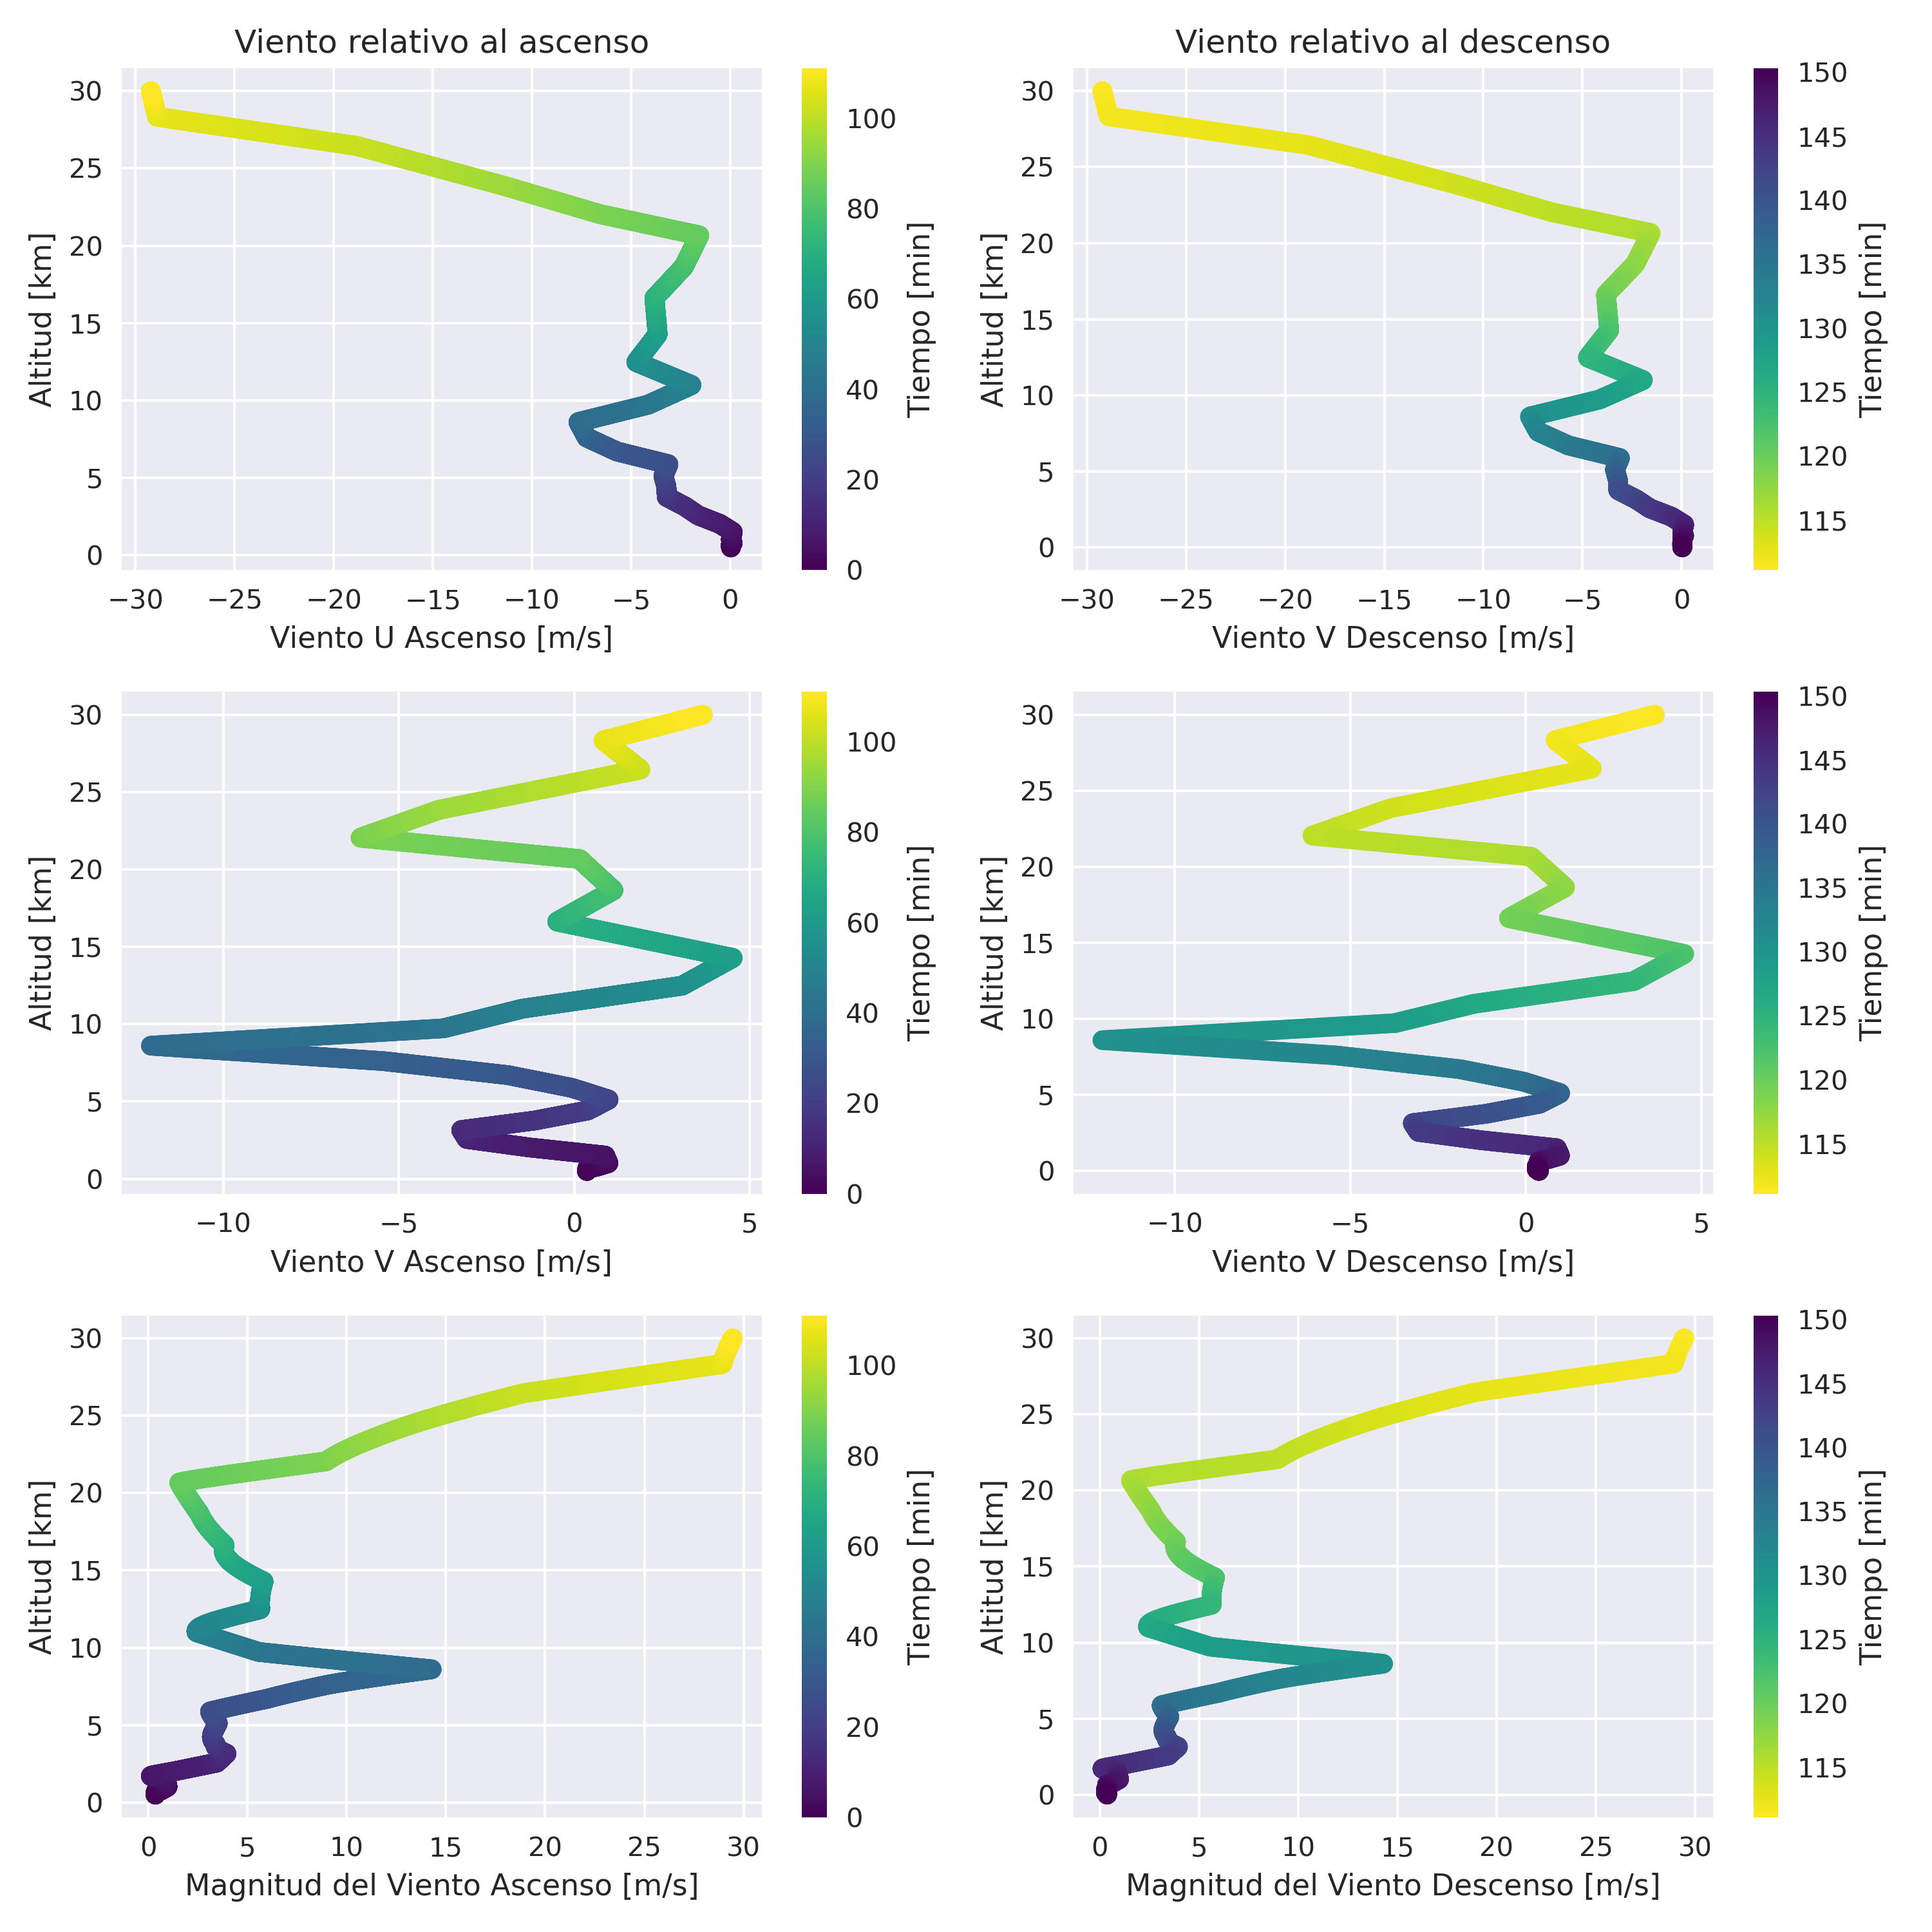
\includegraphics[width=0.85\linewidth]{document/figures/03_vientos.png}
    \caption{Vientos en diferentes planos}
    \label{fig:vientos}
\end{figure}